% ------------------------------------------------------------------------------
% Este fichero es parte de la plantilla LaTeX para la realización de Proyectos
% Final de Grado, protegido bajo los términos de la licencia GFDL.
% Para más información, la licencia completa viene incluida en el
% fichero fdl-1.3.tex

% Copyright (C) 2012 SPI-FM. Universidad de Cádiz
% ------------------------------------------------------------------------------

\documentclass[a4paper,11pt]{book}

% PAQUETES
\usepackage{./estilo/paquetes}
\usepackage{./estilo/colores}
\usepackage{./estilo/comandos}

% Ruta al directorio de imágenes
\graphicspath{{./img/}} 

% METADATOS
\title{AssessMediaWiki}
\author{Jose Alberto Garcia Pinteño}
\date{Septiembre 2015} 
 
\begin{document}

\pagestyle{plain}

% PORTADAS
% ------------------------------------------------------------------------------
% Este fichero es parte de la plantilla LaTeX para la realización de Proyectos
% Final de Grado, protegido bajo los términos de la licencia GFDL.
% Para más información, la licencia completa viene incluida en el
% fichero fdl-1.3.tex

% Copyright (C) 2012 SPI-FM. Universidad de Cádiz
% ------------------------------------------------------------------------------


\begin{titlepage}

  \begin{center}

    
\includegraphics[width=0.3\textwidth]{logo-uca.png} \\
    
    \vspace{2.5cm}
    
    \LARGE{\textbf{ESCUELA SUPERIOR DE INGENIERÍA}} \\
    
    \vspace{1.0cm}
    
    \Large{\textbf{INGENIERÍA TÉCNICA EN INFORMÁTICA DE SISTEMAS}} \\
    
    \vspace{3.0cm}
    
    \Large{PROYECTO DE FIN DE CARRERA} \\
    
    \vspace{2.5cm}
    
    \Large{José Alberto García Pinteño} \\
  
    \vspace{0.5cm}

    \large{\today}
    
  \end{center}
\end{titlepage}

\cleardoublepage

% ------------------------------------------------------------------------------
% Este fichero es parte de la plantilla LaTeX para la realización de Proyectos
% Final de Grado, protegido bajo los términos de la licencia GFDL.
% Para más información, la licencia completa viene incluida en el
% fichero fdl-1.3.tex

% Copyright (C) 2012 SPI-FM. Universidad de Cádiz
% ------------------------------------------------------------------------------


\begin{center}

  
\includegraphics[width=0.3\textwidth]{logo-uca.png} \\

  \vspace{2.5cm}

  \Large{ESCUELA SUPERIOR DE INGENIERÍA} \\

  \vspace{1.0cm}

  \large{INGENIERÍA INFORMÁTICA DE SISTEMAS} \\

  \vspace{2.0cm}

  \large{PROYECTO DE FIN DE CARRERA} \\

  \vspace{2.5cm}

\end{center}

\begin{itemize}
\item \large{Departamento: Ingeniería Informítica}
\item \large{Directores del proyecto: Antonio Balderas Alberico y Manuel Palomo Duarte}
\item \large{Autor del proyecto: José Alberto García Pinteño}
\end{itemize}

\vspace{0.2cm}

\begin{flushright}
  \large{Puerto Real, \today} \\

  \vspace{2.5cm}

  \large{Fdo: José Alberto Garcia Pinteño}
\end{flushright}

\cleardoublepage

% PRELIMINARES
% ------------------------------------------------------------------------------
% Este fichero es parte de la plantilla LaTeX para la realización de Proyectos
% Final de Grado, protegido bajo los términos de la licencia GFDL.
% Para más información, la licencia completa viene incluida en el
% fichero fdl-1.3.tex

% Copyright (C) 2012 SPI-FM. Universidad de Cádiz
% ------------------------------------------------------------------------------

\thispagestyle{empty}

\noindent \textbf{\begin{Large}\textit{Agradecimientos}\end{Large}} 
\newline
\newline
\noindent\textit{Me gustaria darle las gracias a mis padres, ya que sin ellos no podria haber llegado hasta aqui, a mi familia por todo su apoyo y a todos los profesores que se han esforzado por dejar un poco de su conocimiento en mi, en especial a Manuel Palomo, por toda su paciencia y apoyo.}

\newpage

% ------------------------------------------------------------------------------
% Este fichero es parte de la plantilla LaTeX para la realización de Proyectos
% Final de Grado, protegido bajo los términos de la licencia GFDL.
% Para más información, la licencia completa viene incluida en el
% fichero fdl-1.3.tex

% Copyright (C) 2012 SPI-FM. Universidad de Cádiz
% ------------------------------------------------------------------------------

\thispagestyle{empty}

\noindent \textbf{\begin{Large}Resumen\end{Large}} 
\newline
\newline
\noindent

Wiki (del hawaiano wiki, "rápido") es el nombre que recibe un sitio web cuyas páginas pueden ser editadas directamente desde el navegador, donde los usuarios crean, modifican o eliminan contenidos que, generalmente, comparten.
\newline

En este proyecto usaremos los wikis como herramienta docente, permitiendo que los alumnos trabajen sobre el y posteriormente se evalúen entre ellos. Este uso ya esta en practica actualmente, y fue premiado entre los mejores Proyectos de Innovación y Mejora Docente y Proyectos de Innovación Educativa que finalizaron durante el curso 2011/2012. \cite{Balderas:2012}
\newline

 Los wikis son un sistema muy popular como ayuda a la docencia. Cuando el número de estudiantes y la cantidad de información almacenada en un wiki aumentan, evaluar el trabajo de cada estudiante resulta difícil. Los wikis mantienen un registro con las diferencias entre las revisiones consecutivas de los artículos, que pueden ser usadas para la evaluación del aprendizaje. Esta información puede evaluarse a lo largo de la vida del wiki para obtener datos sobre la actividad de los estudiantes.
\newline

AssessMediaWiki es una aplicación web de código abierto que, al conectarse a una instalación MediaWiki, proporciona procedimientos de autoevaluación, hetero evaluación y evaluación entre iguales, a la vez que mantiene información sobre esas evaluaciones. Los supervisores pueden obtener informes que ayudan en la evaluación de los estudiantes.
\newline

Aunque hay un gran número de extensiones para el sistema MediaWiki, no hemos encontrado ninguna que permitiera evaluar contribuciones individuales a un wiki. La mayoría de las aproximaciones solo ofrecen formas de evaluar una versión en particular de un artículo (normalmente la más reciente), siendo ineficaces en este caso. Por ello, para evaluar la calidad de las contribuciones creamos AssessMediaWiki.
\newline

AssessMediaWiki implementa como base dos roles de usuario distintos: supervisores y estudiantes. Los estudiantes pueden elegir entre distintas opciones: evaluar una revisión, comprobar sus propias aportaciones evaluadas y verificar las evaluaciones ya enviadas. Por otro lado, los supervisores tienen un mayor número de opciones, como modificar los parámetros de los programas o vigilar las evaluaciones que los alumnos vayan haciendo.
\newline

\noindent {\bf Palabras clave:} AssessMediaWiki, MediaWiki, Wiki, software libre, evaluación

\newpage


\frontmatter

% INDICES
\tableofcontents
\listoffigures
\listoftables

\mainmatter

\chapter{Introducción}
% ------------------------------------------------------------------------------
% Este fichero es parte de la plantilla LaTeX para la realización de Proyectos
% Final de Grado, protegido bajo los términos de la licencia GFDL.
% Para más información, la licencia completa viene incluida en el
% fichero fdl-1.3.tex

% Copyright (C) 2012 SPI-FM. Universidad de Cádiz
% ------------------------------------------------------------------------------

\section{Motivación}
Tras trabajar durante un breve periodo de tiempo en AssessMediaWiki gracias a la beca Icaro, se planteo la posibilidad de seguir trabajando sobre el mismo, pero esta vez para usarlo como proyecto de fin de carrera.
\newline

Tras esa experiencia, viendo todo lo que había prendido de ella (manejar nuevos lenguajes y herramientas de desarrollo, distintas formas de enfocar los problemas, etc), mi interés por aprender y explorar diversos métodos didácticos y el interés y respeto que tengo hacia el software libre y su comunidad, decidí continuar desarrollando AssessMediaWiki y aprovechar para usarlo como proyecto de fin de carrera, con la posterior motivación extra de intentar hacer publicaciones con el.\\

A medida que desarrollaba el proyecto Manuel Palomo me paso varios artículos de investigación que encontré muy interesantes, tanto por las metodologías aplicadas como por la integración con AssessMediaWiki como es poder medir la participación de los usuarios en las wikis a través de sus sesiones \cite{Stuart} .\\

También me paso otro articulo sobre como afecta visualmente a los usuarios la interfaz y como desarrollar herramientas para mejorar este aspecto en las wikis \cite{Mohamad} lo cual me resulto muy interesante ya que el aspecto visual es uno de los que considero mis puntos débiles.\\

A todo eso también debemos añadirle el privilegio de poder trabajar sobre una de las 10 wikis universitarias mas usadas de España \cite{Ortega} .\\

\section{Alcance} 

Este proyecto está orientado a añadir nuevas herramientas y funciones a AssessMediaWiki, dando un abanico mas amplio de posibilidades a los docentes a la hora de interactuar con los alumnos.

\section{Glosario de Términos} 

\begin{itemize}
	\item AMW - AssessMediaWiki
	\item Edición - Aportación realizada por un alumno al MediaWiki
	\item Metaevaluación - evaluación realizada sobre una evaluación existente, para poder ver así la corrección de la evaluación existente
\end{itemize}

\section{Organización del documento}

En el documento se presenta primero la planificación del desarrollo del sistema, así como la metodología de trabajo a seguir.
\newline

En el apartado de desarrollo se muestran un análisis de requisitos y de el sistema actual. También se mesta el proceso para la implementación de las nuevas funciones, así como las modificaciones en las bases de datos.
\newline

En la parte final del documento encontramos el epilogo con el manual de instalación, el manual de uso y la bibliografía utilizada en este documento.





\chapter{Planificación}
% ------------------------------------------------------------------------------
% Este fichero es parte de la plantilla LaTeX para la realización de Proyectos
% Final de Grado, protegido bajo los términos de la licencia GFDL.
% Para más información, la licencia completa viene incluida en el
% fichero fdl-1.3.tex

% Copyright (C) 2012 SPI-FM. Universidad de Cádiz
% ------------------------------------------------------------------------------


\section{Metodología de desarrollo}
Definición del proceso de desarrollo, ciclo de vida y metodología empleada durante la elaboración del proyecto. Las fases y/o iteraciones que proponga el método empleado deberán quedar recogidas en la planificación que se detalle más adelante.

Se ha optado por una metodología de desarrollo en cascada, como se aprecia en la siguiente imagen:

\begin{figure}[h!]
	\centering
	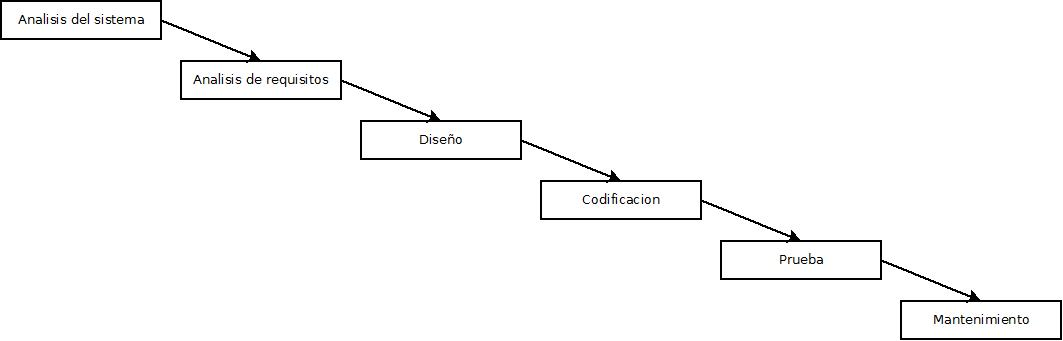
\includegraphics[width=1.0\textwidth]{Cascada.jpg}
	\caption{Desarrollo en cascada.}
\end{figure}

\section{Planificación del proyecto}
Estimación temporal y definición del calendario básico (hitos principales e iteraciones). Desarrollo de la planificación detallada, utilizando un diagrama de Gantt.\\

Se debe incluir una comparación cuantitativa del tiempo y el esfuerzo realmente invertido frente al estimado y planificado. Estos datos pueden recogerse del sistema de gestión de tareas empleado para el seguimiento del proyecto.


\begin{figure}[h]
	\centering
	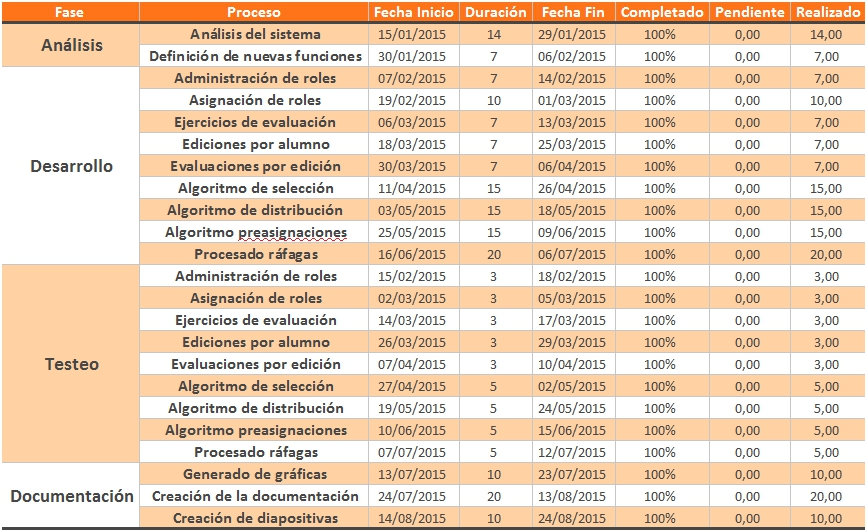
\includegraphics[width=1.0\textwidth]{Gantt-numerico.jpg}
	\caption{Datos del diagrama de Gantt.}
\end{figure}

\begin{figure}[h!]
	\centering
	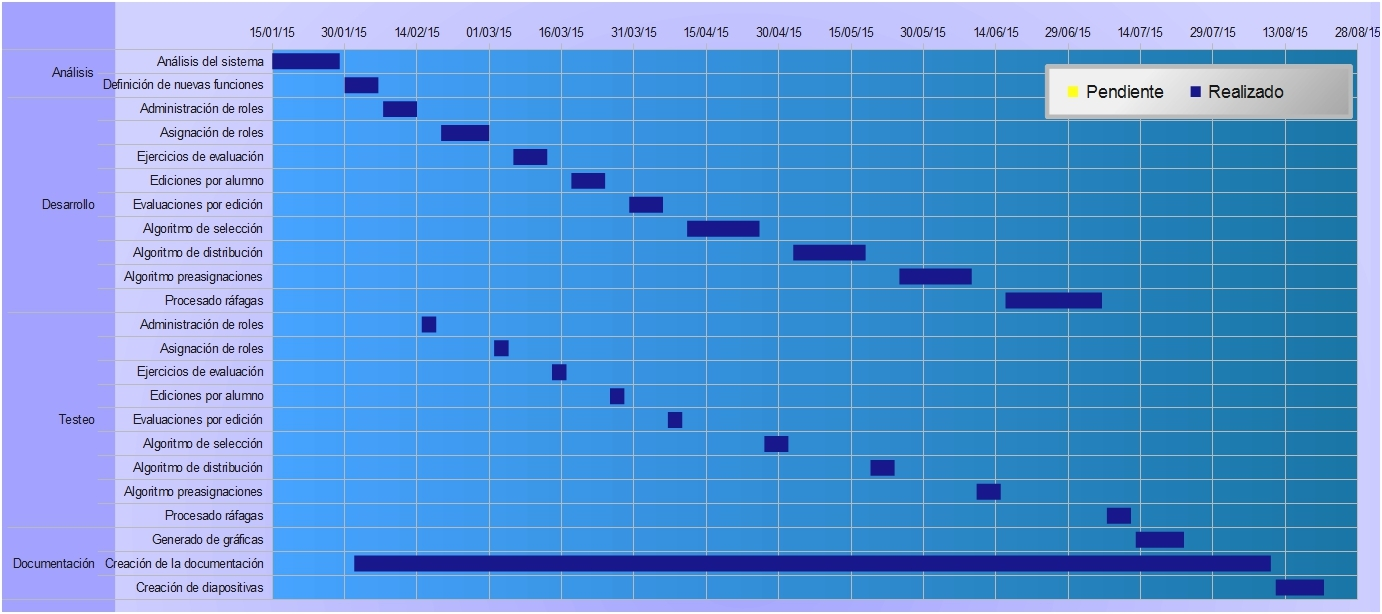
\includegraphics[width=1.0\textwidth]{Gantt-grafica.jpg}
	\caption{Diagrama de Gantt.}
\end{figure}


\begin{figure}[h!]
	\centering
	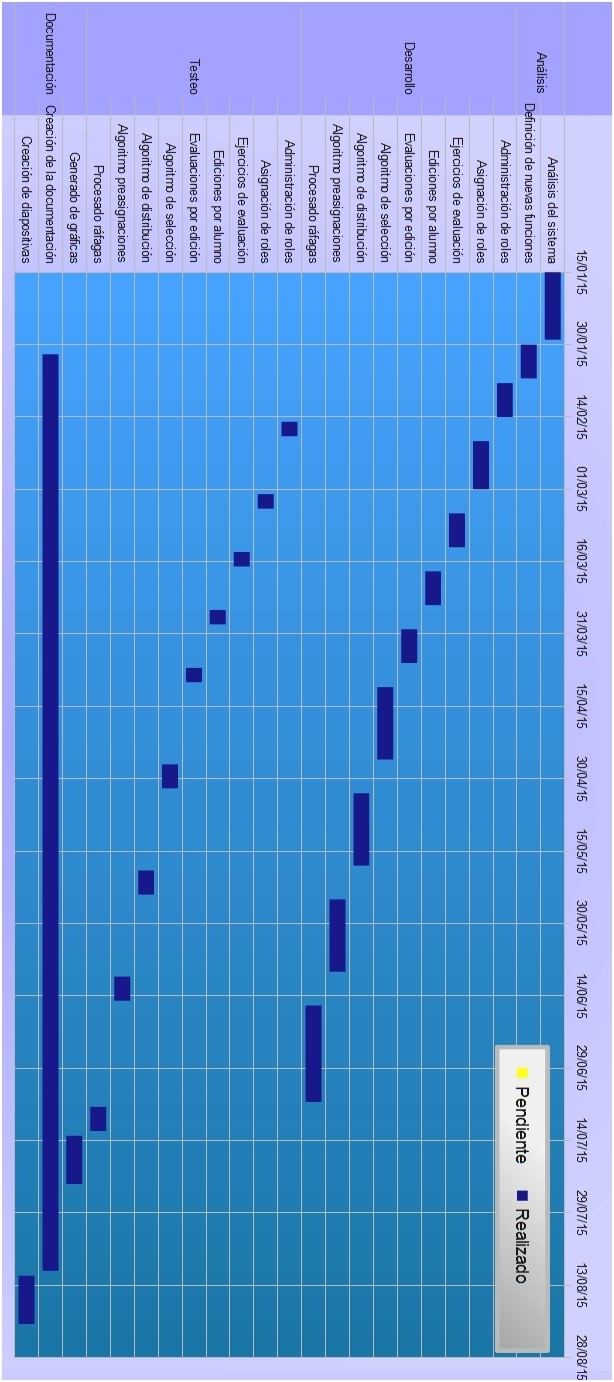
\includegraphics[width=0.6\textwidth]{Gantt-grafica-girada.jpg}
	\caption{Diagrama de Gantt (girada).}
\end{figure}

\clearpage

\section{Organización}
Relación de las personas (roles) involucradas en el proyecto y de cómo se estructuran las relaciones entre las mismas para ejecutar el proyecto. Relación de los recursos inventariables utilizados en el proyecto: equipamiento informático (hardware y software), herramientas empleadas, etc. \\

Para llevar a cabo este proyecto es necesario un MediaWiki. un servidor para alojar AssessMediaWiki y en caso de que el profesor no posea los conocimientos necesarios para la instalación, la colaboración de personal que facilite la instalación de AssessMediaWiki

\section{Riesgos}
Enumeración de los riesgos del proyecto, indicando su posible impacto (efecto que la ocurrencia del citado riesgo tendría en el desarrollo del proyecto) y la probabilidad de ocurrencia. Una vez los riesgos son identificados y priorizados, hay que definir los planes necesarios para reducir los efectos del riesgo una vez se haya materializado o disminuir que este ocurra.\\

De momento hay un pequeño problema con los nombres de los roles creados en el sistema AssessMediaWiki y los ejercicios de evaluación, si los nombres llevan espacio no se podrán eliminar, y es posible que no puedan ser modificados, es un pequeño detalle que se puede arreglar en un trabajo futuro, para evitar este problema basta con usar barras bajas en lugar de espacios.\\

También puede considerarse un riesgo usar el framework (\href{http://www.codeigniter.com/}{CodeIgniter}) sin conocimiento previo, así como que en un futuro dicho framework deje de recibir soporte.


% DESARROLLO
\part{Desarrollo}

\chapter{Requisitos del Sistema}
% ------------------------------------------------------------------------------
% Este fichero es parte de la plantilla LaTeX para la realización de Proyectos
% Final de Grado, protegido bajo los términos de la licencia GFDL.
% Para más información, la licencia completa viene incluida en el
% fichero fdl-1.3.tex

% Copyright (C) 2012 SPI-FM. Universidad de Cádiz
% ------------------------------------------------------------------------------


\section{Situación actual} 
En la versión actual (la que esta funcionando en estos momentos) de AssessMediaWiki nos encontramos con un algoritmo de selección que escoge una edición de forma aleatoria entre las $n$ ediciones mas significativas (las de mayor tamaño), de forma que en el peor de los casos nos encontramos con la situación de que las $n-1$ ediciones mas significativas nunca serán seleccionadas.
\newline
Esta versión de AssessMediaWiki también carece de un procesado de ediciones para ciertos wiki-comportamientos (ráfagas, correcciones ortográficas, etc) y los roles de los usuarios se limitan a los de alumno y supervisor.\\
Estos situaciones han sido complementadas con esta nueva versión, añadiendo un algoritmo distinto de selección de ediciones, un sistema de administración de roles y el procesado de ráfagas

\subsection{Entorno Tecnológico}
Para este proyecto sera necesario contar con un MediaWiki, normalmente alojado en un servidor, en el cual seria recomendable alojar el mismo software del proyecto.

\subsection{Fortalezas y Debilidades}
Fortalezas: Herramienta muy útil para añadir nuevas posibilidades a los métodos docentes.//

Debilidades: Es necesario un mínimo de conocimientos para su instalación, al igual que para la instalación del MediaWiki.

\section{Objetivos del Sistema}
El objetivo del sistema es añadir nuevas funciones al método docente y darle a los alumnos mas responsabilidades, así como analizar su participación y resultados.

\section{Catálogo de Requisitos}

\subsection{Requisitos funcionales}
Listado de las nuevas funcionalidades que ofrece el sistema:

\begin{itemize}
	\item Creación y edición de nuevos roles.
	\item Creación y edición de ejercicios de evaluación.
	\item Procesado de ráfagas.
	\item Preasignaciones de ediciones.
\end{itemize}

\subsection{Requisitos no funcionales}
Descripción de otros requisitos (relacionados con la calidad del software) que el sistema deberá satisfacer: portabilidad, seguridad, estándares de obligado cumplimiento, accesibilidad, usabilidad, etc:
\begin{itemize}
	\item MediaWiki.
	\item Servidor para hospedar tanto el MediaWiki como AssessMediaWiki.
	\item Conexión a internet.
\end{itemize}

\subsection{Requisitos de información}
En esta sección se describen los requisitos de gestión de información (datos) que el sistema debe gestionar:
\begin{itemize}
	\item IDs de los usuarios del MediaWiki.
	\item IDs de las ediciones creadas por los usuarios.
	\item Notas y comentarios asignados a ediciones evaluadas.
	\item Parámetros de configuración
	\item Roles creados por el administrador.
	\item Ejercicios de evaluación y sus configuraciones.
\end{itemize}

\section{Alternativas de Solución}
Se presento la posibilidad de usar Eval-comix[] como herramienta de evaluación alternativa.

\section{Solución Propuesta}
Se descartó usar Eval-comix[] debido a que se consideró mejor opción implementar un método propio que fuese escalable.

\chapter{Análisis del Sistema}
% ------------------------------------------------------------------------------
% Este fichero es parte de la plantilla LaTeX para la realización de Proyectos
% Final de Grado, protegido bajo los términos de la licencia GFDL.
% Para más información, la licencia completa viene incluida en el
% fichero fdl-1.3.tex

% Copyright (C) 2012 SPI-FM. Universidad de Cádiz
% ------------------------------------------------------------------------------


\section{Modelo Conceptual}

A partir de los requisitos de información, se desarrollará un diagrama conceptual de clases UML, identificando las clases, atributos, relaciones, restricciones adicionales y reglas de derivación necesarias, primero describiremos tas tablas y los atributos de la bases bases de datos (la antigua y la de la nueva versión).\\

\textbf{Base de datos 1.0}\\

\begin{itemize}	
	\item Config\\
	
	En esta tabla almacenaremos los parámetros de las configuraciones.
	
	\begin{itemize}
		\item parameter - nombre del parámetro
		\item value - valor del parámetro
	\end{itemize}
	
	\item Entregables\\
	
	En esta tabla almacenaremos las categorías a evaluar en cada ejercicio.
	
	\begin{itemize}
		\item ent id - id de la categoría a evaluar
		\item ent entregale - nombre de la categoría a evaluar
		\item ent descripción - descripción de la categoría a evaluar
	\end{itemize}
	
	\item Evaluaciones\\
	
	En esta tabla almacenaremos datos de la edición evaluada.
	
	\begin{itemize}
		\item eva id - id de la evaluación
		\item eva user - id del autor de la edición
		\item eva revisor - id del evaluador de la edición
		\item eva revision - id de la edición
		\item eva time - tiempo empleado en la evaluación
	\end{itemize}
	
	\item Evaluaciones entregables\\
	
	En esta tabla almacenaremos los datos de la evaluación.
	
	\begin{itemize}
		\item eva id - id de la evaluación
		\item ent id - id de la categoría evaluada
		\item ee nota - nota de la edición en una categoría
		\item ee comentario - comentarios sobre la valoración de la edición
	\end{itemize}
	
	\item Metaevaluaciones\\
	
	En esta tabla almacenaremos las metaevaluaciones realizadas.
	
	\begin{itemize}
		\item mev id - id de la metaevaluación
		\item mevaluador id - id del meta-evaluador
		\item evaluación id - id de la evaluación
		\item calificación - valoración de la evaluación
		\item comentario - comentarios sobre la valoración de la evaluación
	\end{itemize}
	
	
	\item Replies\\
	
	En esta tabla almacenaremos las re-evaluaciones solicitadas.
	
	\begin{itemize}
		\item rep id - id del reply
		\item rep read - id de la evaluación antigua
		\item rep new - id de la nueva evaluación
	\end{itemize}
	

	
\end{itemize}

\begin{figure} [h]
	\centering
	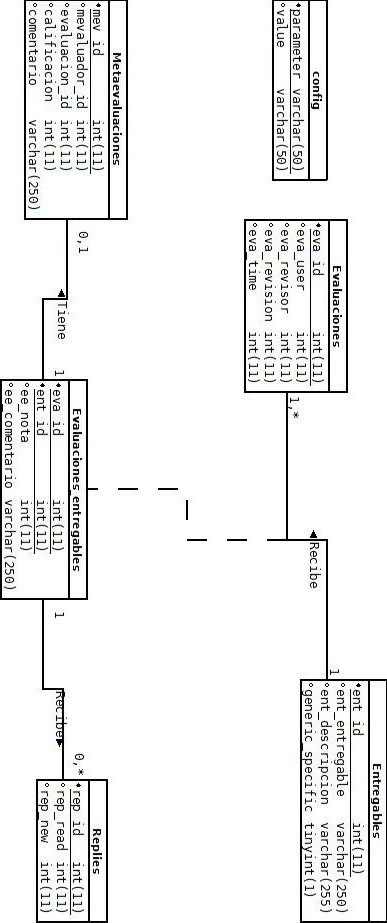
\includegraphics[width=0.6\textwidth]{db1girada.jpg}
	\caption{Diagrama de la base de datos de AMW 1.0.}
\end{figure}

\clearpage

\textbf{Base de datos 2.0}\\
	
\begin{itemize}
	\item Categorías ej ev\\
	
	En esta tabla almacenaremos información de las categorías de los ejercicios de evaluación.\\
	
	\begin{itemize}
		\item evaluation id - id del ejercicio de evaluación
		\item ent id - id de la categoría a evaluar
	\end{itemize}
	
	\item Config\\
	
	En esta tabla almacenaremos los parámetros de las configuraciones.
	
	\begin{itemize}
		\item parameter - nombre del parámetro
		\item value - valor del parámetro
	\end{itemize}
	
	\item Ejercicios de evaluación\\
	
	En esta tabla almacenaremos los distintos ejercicios de evaluación.
	
	\begin{itemize}
		\item evaluation id - id del ejercicio de evaluación
		\item exercise name - nombre del ejercicio de evaluación
		\item beginning - fecha de inicio
		\item first phase end - fin del periodo de definición de los criterios de evaluación
		\item second phase end - fin del periodo de desarrollo del ejercicio
		\item third phase end - fin del periodo de evaluación entre alumnos
		\item fourth phase end - fin de la fase final de supervisión
		\item description - descripción del ejercicio de evaluación
	\end{itemize}
	
	\item Entregables\\
	
	En esta tabla almacenaremos las categorías a evaluar en cada ejercicio.
	
	\begin{itemize}
		\item ent id - id de la categoría a evaluar
		\item ent entregale - nombre de la categoría a evaluar
		\item ent descripción - descripción de la categoría a evaluar
		\item generic specific - define si la categoría a evaluar es genérica o especifica
	\end{itemize}
	
	\item Evaluaciones\\
	
	En esta tabla almacenaremos datos de la edición una vez haya sido evaluada.
	
	\begin{itemize}
		\item eva id - id de la evaluación
		\item eva user - id del autor de la edición
		\item eva revisor - id del evaluador de la edición
		\item eva revision - id de la edición
		\item eva time - tiempo empleado en la evaluación
	\end{itemize}
	
	\item Evaluaciones entregables\\
	
	En esta tabla almacenaremos los datos de la evaluación.
	
	\begin{itemize}
		\item eva id - id de la evaluación
		\item ent id - id de la categoría evaluada
		\item ee nota - nota de la edición en una categoría
		\item ee comentario - comentarios sobre la valoración de la edición
	\end{itemize}
	
	\item Metaevaluaciones\\
	
	En esta tabla almacenaremos las metaevaluaciones realizadas.
	
	\begin{itemize}
		\item mev id - id de la metaevaluación
		\item mevaluador id - id del meta-evaluador
		\item evaluación id - id de la evaluación
		\item calificación - valoración de la evaluación
		\item comentario - comentarios sobre la valoración de la evaluación
	\end{itemize}
	
	\item Preasignaciones\\
	
	En esta tabla almacenaremos las preasignaciones realizadas.
	
	\begin{itemize}
		\item preasignación id - id de la preasignación
		\item edit id - id de la edición
		\item revisor id - id del evaluador de la edición
		\item ejercicio de evaluación - id del ejercicio de evaluación
	\end{itemize}
	
	\item Ráfagas\\
	
	En esta tabla almacenaremos las ráfagas de ediciones generadas.
	
	\begin{itemize}
		\item raf start - id de la edición donde empieza la ráfaga
		\item raf end - id de la edición donde termina la ráfaga
		\item raf timestamp - fecha y hora de la edición final
		\item raf size - tamaño de la ráfaga
	\end{itemize}
	
	\item Replies\\
	
	En esta tabla almacenaremos las re-evaluaciones solicitadas.
	
	\begin{itemize}
		\item rep id - id del reply
		\item rep read - id de la evaluación antigua
		\item rep new - id de la nueva evaluación
	\end{itemize}
	
	\item Rol assignations\\
	
	En esta tabla almacenaremos las asignaciones de roles.
	
	\begin{itemize}
		\item user id - id del usuario
		\item rol id - id del rol
	\end{itemize}
	
	\item Roles\\
	
	En esta tabla almacenaremos los roles existentes.
	
	\begin{itemize}
		\item rol id - id del rol
		\item name - nombre del rol
		\item evaluar - permisos para la sección de evaluar
		\item feedback - permisos para la sección de feedback
		\item metaevaluar - permisos para la sección de metaevaluar
		\item metaevaluar lista - permisos para la sección de la lista de metaevaluaciones
		\item alumnos - permisos para la sección de la lista de alumnos
		\item parámetros - permisos para la sección de parámetros
	\end{itemize}
	
\end{itemize}

\begin{figure}[h]
	\centering
	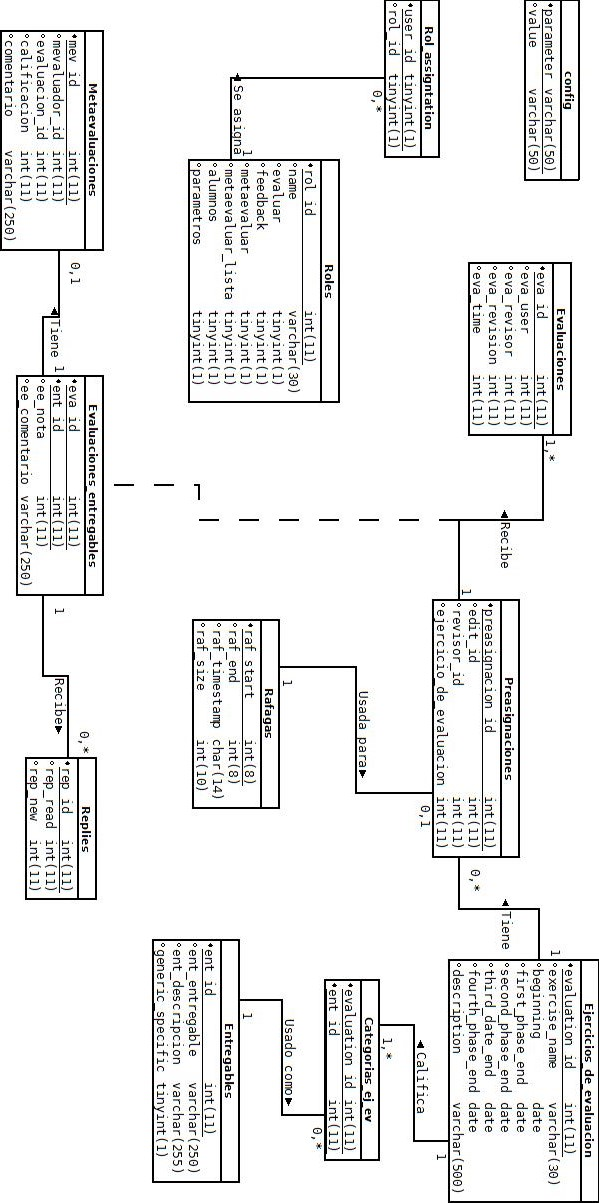
\includegraphics[width=0.6\textwidth]{db2girada.jpg}
	\caption{Diagrama de la base de datos de AMW 2.0.}
\end{figure}

\clearpage

\section{Modelo de Casos de Uso}

\begin{figure}
	\centering
	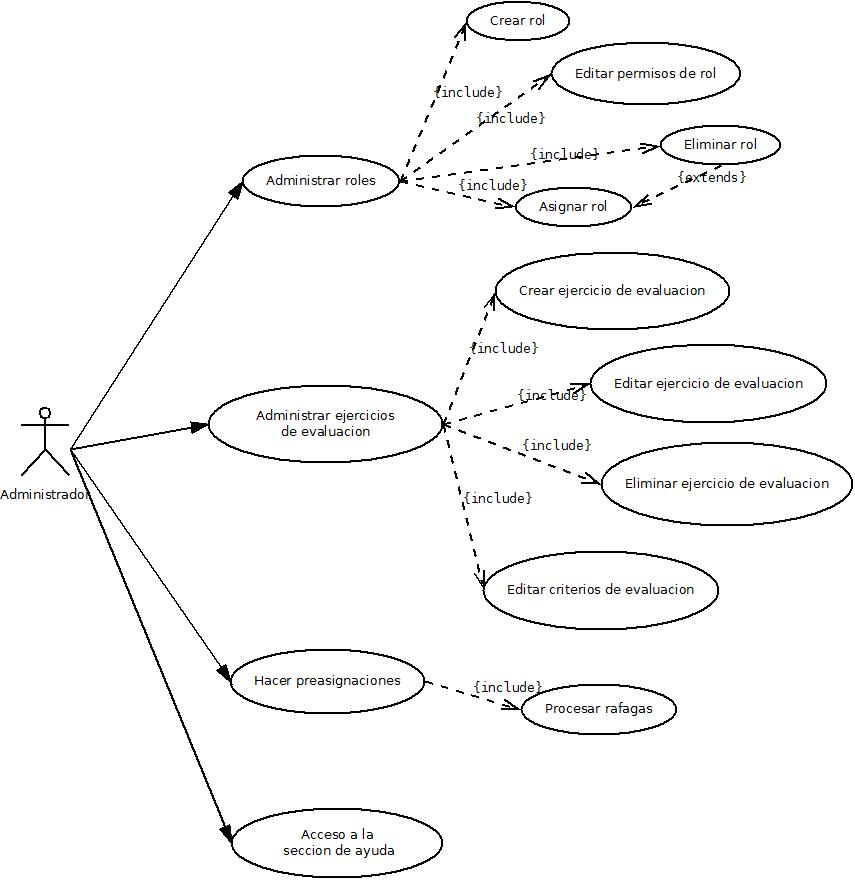
\includegraphics[width=1.0\textwidth]{Casos-de-uso.jpg}
	\caption{Modelo de casos de uso.}
\end{figure}

\subsection{Actores} 
Los actores básicos son:
\newline
- Administrador/Profesor: El usuario supervisor del sistema
\newline
- Estudiante: Usuario que realizara las evaluaciones de las ediciones suyas o de sus compañeros
\newline

Pero hay que tener en cuenta que el administrador puede crear nuevos roles, lo que generara nuevos actores dependiendo de los permisos que se les conceda a dichos roles.

\newpage

\subsection{Descripción de los casos de uso}
Caso de uso:  \textbf{Administrar roles}
\newline
Descripción: El usuario se dirige a la pagina de administración de roles.
\newline
Actores: Usuario, Sistema
\newline
Precondiciones: El usuario esta logeado y es administrador.
\newline
Postcondiciones: El sistema muestra la pagina de administración de roles.
\newline
Escenario principal:
\begin{itemize}
	\item 1. El usuario hace clic en el enlace a la administración de roles.
	\item El sistema muestra la pagina de administración de roles.
\end{itemize}

Escenario alternativo 1: 
\begin{itemize}
	\item *.* En cualquier momento del caso de uso el usuario usa los botones de navegación (atrás, adelante, actualizar) y termina el proceso actual sin guardar los datos ni ejecutarse ninguna acción.
\end{itemize}
Escenario alternativo 2:
\begin{itemize}
\item *.* En cualquier momento del caso de uso el usuario viaja a otra sección de la web o a otra web y termina el proceso actual sin guardar los datos ni ejecutarse ninguna acción.
\end{itemize}

Caso de uso: \textbf{Crear rol}
\newline
Descripción: El usuario decide crear un nuevo rol.
\newline
Actores: Usuario, Sistema
\newline
Precondiciones: El usuario esta logeado y es administrador y se encuentra en la pagina de administración de roles.
\newline
Postcondiciones: Se introduce un nuevo rol en la base de datos del sistema.
\newline
Escenario principal:
\begin{itemize}
	\item 1. El usuario rellena los datos para crear un nuevo rol en la pagina de administración de roles.
	\item 2. El usuario hace clic en crear rol.
	\item 3. El sistema comprueba que no existe ningún otro rol en el sistema con el nombre del nuevo rol a crear.
	\item 4. El sistema añade el nuevo rol a la base de datos del sistema.
 \item 5. El sistema actualiza la pagina de administración de roles, mostrando también el nuevo rol añadido.
\end{itemize}
Escenario alternativo 1: 
\begin{itemize}
	\item *.* En cualquier momento del caso de uso el usuario usa los botones de navegación (atrás, adelante, actualizar) y termina el proceso actual sin guardar los datos ni ejecutarse ninguna acción.
\end{itemize}
Escenario alternativo 2:
\begin{itemize}
	\item *.* En cualquier momento del caso de uso el usuario viaja a otra sección de la web o a otra web y termina el proceso actual sin guardar los datos ni ejecutarse ninguna acción.
\end{itemize}
Escenario alternativo 3:
\begin{itemize}
	\item 3.a El sistema detecta que el nuevo rol a introducir ya existe en el sistema.
	\item 4.a El sistema actualiza la pagina de administración de roles, sin añadir el nuevo rol que el usuario pretendía añadir.
\end{itemize}

Caso de uso: \textbf{Editar permisos de rol}
\newline
Descripción: El usuario decide editar los permisos de un rol.
\newline
Actores: Usuario, Sistema
\newline
Precondiciones: El usuario esta logeado y es administrador y se encuentra en la pagina de administración de roles.
\newline
Postcondiciones: Se modifican los permisos de un rol en la base de datos del sistema.
\newline
Escenario principal:
\begin{itemize}
\item 1. El usuario rellena los datos para modificar los permisos de un rol en la pagina de administración de roles.
\item 2. El usuario hace clic en modificar rol.
\item 3. El sistema modifica los permisos del rol en la base de datos del sistema.
\item 4. El sistema actualiza la pagina de administración de roles, mostrando los cambios efectuados.
\end{itemize}
Escenario alternativo 1: 
\begin{itemize}
	\item *.* En cualquier momento del caso de uso el usuario usa los botones de navegación (atrás, adelante, actualizar) y termina el proceso actual sin guardar los datos ni ejecutarse ninguna acción.
\end{itemize}
Escenario alternativo 2:
\begin{itemize}
	\item *.* En cualquier momento del caso de uso el usuario viaja a otra sección de la web o a otra web y termina el proceso actual sin guardar los datos ni ejecutarse ninguna acción.
\end{itemize}

Caso de uso: \textbf{Eliminar rol}
\newline
Descripción: El usuario decide eliminar rol.
\newline
Actores: Usuario, Sistema
\newline
Precondiciones: El usuario esta logeado y es administrador y se encuentra en la pagina de administración de roles.
\newline
Postcondiciones: Se elimina el rol seleccionado de la base de datos del sistema.
\newline
Escenario principal:
\begin{itemize}
	\item 1. El sistema muestra una lista desplegable con los roles existentes en el sistema, exceptuando los de administrador y estudiante.
	\item 2. El usuario selecciona el rol que desea eliminar.
	\item 3. El usuario hace clic en el botón de eliminar rol.
	\item 4. El sistema elimina todas las asignaciones de usuarios al rol a eliminar.
	\item 5. El sistema elimina el rol seleccionado de la base de datos del sistema.
	\item 6. El sistema actualiza la pagina de administración de roles, mostrando los cambios efectuados.
\end{itemize}
Escenario alternativo 1:
\begin{itemize} 
	\item *.* En cualquier momento del caso de uso el usuario usa los botones de navegación (atrás, adelante, actualizar) y termina el proceso actual sin guardar los datos ni ejecutarse ninguna acción.
\end{itemize}
Escenario alternativo 2:
\begin{itemize}
	\item *.* En cualquier momento del caso de uso el usuario viaja a otra sección de la web o a otra web y termina el proceso actual sin guardar los datos ni ejecutarse ninguna acción.
\end{itemize}

Caso de uso: \textbf{Asignar rol}
\newline
Descripción: El usuario decide asignar un rol a un estudiante.
\newline
Actores: Usuario, Sistema
\newline
Precondiciones: El usuario esta logeado y es administrador y se encuentra en la pagina de administración de roles.
\newline
Postcondiciones: Se introduce un nuevo rol en la base de datos del sistema.
\newline
Escenario principal:
\begin{itemize}
	\item 1. El sistema muestra una lista desplegable con los usuarios existentes en el sistema y otra con los roles existentes en el sistema.
	\item 2. El usuario selecciona un usuario y un rol de las listas.
	\item 3. El usuario hace clic en el botón de asignar rol.
	\item 4. El sistema comprueba que el usuario no tenia ningún rol asignado.
	\item 5. El sistema introduce los datos del usuario seleccionado y el rol que se le va a asignar.
	\item 6. El sistema actualiza la pagina de administración de roles, mostrando los cambios efectuados.
\end{itemize}
Escenario alternativo 1: 
\begin{itemize}
	\item *.* En cualquier momento del caso de uso el usuario usa los botones de navegación (atrás, adelante, actualizar) y termina el proceso actual sin guardar los datos ni ejecutarse ninguna acción.
\end{itemize}
Escenario alternativo 2:
\begin{itemize}
	\item *.* En cualquier momento del caso de uso el usuario viaja a otra sección de la web o a otra web y termina el proceso actual sin guardar los datos ni ejecutarse ninguna acción.
\end{itemize}
Escenario alternativo 3:
\begin{itemize}
	\item 4.a El sistema detecta que el usuario ya tiene un rol asignado.
	\item 5.a El sistema detecta que el nuevo rol que se le quiere asignar es el de estudiante.
	\item 7.a El sistema borra de la base de datos la asignación previa que tuviera el usuario seleccionado.
	\item 8.a El sistema actualiza la pagina de administración de roles, mostrando los cambios efectuados.
\end{itemize}
Escenario alternativo 4:
\begin{itemize}
	\item 5.b El sistema detecta que el nuevo rol que se quiere asignar no es el de estudiante.
	\item 6.b El sistema actualiza la base de datos con los nuevos datos introducidos
	\item 7.b El sistema actualiza la pagina de administración de roles mostrando los cambios efectuados.
\end{itemize}

Caso de uso: \textbf{Administrar ejercicios de evaluación}
\newline
Descripción: El usuario se dirige a la pagina de administración de ejercicios de evaluación
\newline
Actores: Usuario, Sistema
\newline
Precondiciones: El usuario esta logeado y es administrador.
\newline
Postcondiciones: El sistema muestra la pagina de administración de ejercicios de evaluación
\newline
Escenario principal:
\begin{itemize}
	\item 1. El usuario hace clic en el enlace a la administración de ejercicios de evaluación
	\item 2. El sistema muestra la pagina de administración de ejercicios de evaluación
\end{itemize}
Escenario alternativo 1: 
\begin{itemize}
	\item *.* En cualquier momento del caso de uso el usuario usa los botones de navegación (atrás, adelante, actualizar) y termina el proceso actual sin guardar los datos ni ejecutarse ninguna acción.
\end{itemize}
Escenario alternativo 2: 
\begin{itemize}
	\item *.* En cualquier momento del caso de uso el usuario viaja a otra sección de la web o a otra web y termina el proceso actual sin guardar los datos ni ejecutarse ninguna acción.
\end{itemize}

Caso de uso: \textbf{Crear ejercicio de evaluación}
\newline
Descripción: El usuario decide crear un nuevo ejercicio de evaluación
\newline
Actores: Usuario, Sistema
\newline
Precondiciones: El usuario esta logeado y es administrador y se encuentra en la pagina de administración de ejercicios de evaluación
\newline
Postcondiciones: Se introduce un nuevo ejercicio de evaluación en la base de datos del sistema.
\newline
Escenario principal:
\begin{itemize}
	\item 1. El usuario rellena los datos para crear un nuevo ejercicio de evaluación en la pagina de administración de ejercicios de evaluación
	\item 2. El usuario hace clic en crear ejercicio de evaluación
	\item 3. El sistema comprueba que no existe ningún otro ejercicio de evaluación en el sistema con el nombre del nuevo ejercicio de evaluación a crear.
	\item 4. El sistema añade el nuevo ejercicio de evaluación a la base de datos del sistema.
	\item 5. El sistema actualiza la pagina de administración de ejercicios de evaluación, mostrando también el nuevo ejercicio de evaluación añadido.
\end{itemize}
Escenario alternativo 1: 
\begin{itemize}
	\item *.* En cualquier momento del caso de uso el usuario usa los botones de navegación (atrás, adelante, actualizar) y termina el proceso actual sin guardar los datos ni ejecutarse ninguna acción.
\end{itemize}
Escenario alternativo 2:
\begin{itemize}
	\item *.* En cualquier momento del caso de uso el usuario viaja a otra sección de la web o a otra web y termina el proceso actual sin guardar los datos ni ejecutarse ninguna acción.
\end{itemize}
Escenario alternativo 3:
\begin{itemize}
	\item 3.a El sistema detecta que el nuevo ejercicio de evaluación a introducir ya existe en el sistema.
	\item 4.a El sistema actualiza la pagina de administración de ejercicios de evaluación, sin añadir el nuevo ejercicio de evaluación que el usuario pretendía añadir.
\end{itemize}

Caso de uso: \textbf{Editar ejercicio de evaluación}
\newline
Descripción: El usuario decide editar un ejercicio de evaluación
\newline
Actores: Usuario, Sistema
\newline
Precondiciones: El usuario esta logeado y es administrador y se encuentra en la pagina de administración de ejercicios de evaluación
\newline
Postcondiciones: Se modifican un ejercicio de evaluación en la base de datos del sistema.
\newline
Escenario principal:
\begin{itemize}
	\item 1. El usuario rellena los datos para modificar un ejercicio de evaluación en la pagina de administración de roles.
	\item 2. El usuario hace clic en modificar ejercicio de evaluación
	\item 4. El sistema modifica el ejercicio de evaluación en la base de datos del sistema.
	\item 5. El sistema actualiza la pagina de administración de ejercicios de evaluación, mostrando los cambios efectuados.
\end{itemize}
Escenario alternativo 1: 
\begin{itemize}
	\item *.* En cualquier momento del caso de uso el usuario usa los botones de navegación (atrás, adelante, actualizar) y termina el proceso actual sin guardar los datos ni ejecutarse ninguna acción.
\end{itemize}
Escenario alternativo 2:
\begin{itemize}
	\item *.* En cualquier momento del caso de uso el usuario viaja a otra sección de la web o a otra web y termina el proceso actual sin guardar los datos ni ejecutarse ninguna acción.
\end{itemize}

Caso de uso: \textbf{Eliminar ejercicio de evaluación}
\newline
Descripción: El usuario decide eliminar un ejercicio de evaluación
\newline
Actores: Usuario, Sistema
\newline
Precondiciones: El usuario esta logeado y es administrador y se encuentra en la pagina de administración de ejercicio de evaluación
\newline
Postcondiciones: Se elimina el ejercicio de evaluación seleccionado de la base de datos del sistema.
\newline
Escenario principal:
\begin{itemize}
	\item 1. El sistema muestra una lista desplegable con los ejercicios de evaluación existentes en el sistema.
	\item 2. El usuario selecciona el ejercicio de evaluación que desea eliminar.
	\item 3. El usuario hace clic en el botón de eliminar ejercicio de evaluación
	\item 4. El sistema elimina el ejercicio de evaluación seleccionado de la base de datos del sistema.
	\item 5. El sistema actualiza la pagina de administración de ejercicios de evaluación, mostrando los cambios efectuados.
\end{itemize}
Escenario alternativo 1: 
\begin{itemize}
	\item *.* En cualquier momento del caso de uso el usuario usa los botones de navegación (atrás, adelante, actualizar) y termina el proceso actual sin guardar los datos ni ejecutarse ninguna acción.
\end{itemize}
Escenario alternativo 2:
\begin{itemize}
	\item *.* En cualquier momento del caso de uso el usuario viaja a otra sección de la web o a otra web y termina el proceso actual sin guardar los datos ni ejecutarse ninguna acción.
\end{itemize}

Caso de uso: \textbf{Editar criterios de evaluación}
\newline
Descripción: El usuario decide editar los criterios de evaluación de un ejercicio de evaluación
\newline
Actores: Usuario, Sistema
\newline
Precondiciones: El usuario esta logeado y es administrador y se encuentra en la pagina de administración de ejercicio de evaluación
\newline
Postcondiciones: Se modifican los criterios de evaluación de un ejercicio de evaluación en la base de datos del sistema.
\newline
Escenario principal:
\begin{itemize}
	\item 1. El sistema muestra una tabla con los ejercicio de evaluación y criterios de evaluación existentes en el sistema.
	\item 2. El usuario modifica los criterios de evaluación de uno de los ejercicios de evaluación
	\item 3. El usuario hace clic en el botón de modificar criterios de evaluación
	\item 4. El sistema modifica los datos para el ejercicio de evaluación seleccionado.
	\item 5. El sistema actualiza la pagina de administración de roles, mostrando los cambios efectuados.
\end{itemize}
Escenario alternativo 1: 
\begin{itemize}
	\item *.* En cualquier momento del caso de uso el usuario usa los botones de navegación (atrás, adelante, actualizar) y termina el proceso actual sin guardar los datos ni ejecutarse ninguna acción.
\end{itemize}
Escenario alternativo 2:
\begin{itemize}
	\item *.* En cualquier momento del caso de uso el usuario viaja a otra sección de la web o a otra web y termina el proceso actual sin guardar los datos ni ejecutarse ninguna acción.
\end{itemize}

Caso de uso: \textbf{Hacer Preasignaciones}
\newline
Descripción: El usuario decide realizar las preasignaciones para un ejercicio de evaluación
\newline
Actores: Usuario, Sistema
\newline
Precondiciones: El usuario esta logeado y es administrador y se encuentra en la pagina de administración de ejercicio de evaluación
\newline
Postcondiciones: Se realizan las preasignaciones para un ejercicio de evaluación
\newline
Escenario principal:
\begin{itemize}
	\item 1. El sistema muestra una lista desplegable con los ejercicio de evaluación para los cuales aun no se han realizado preasignaciones existentes en el sistema.
	\item 2. El usuario selecciona uno de los ejercicios de evaluación
	\item 3. El usuario hace clic en el botón de hacer preasignaciones
	\item 4. El sistema realiza el procesado de ráfagas y posteriormente asigna las ediciones del ejercicio de evaluación a los Estudiantes según la configuración del sistema.
	\item 5. El sistema actualiza la pagina de administración de ejercicios de evaluación, mostrando los cambios efectuados.
\end{itemize}
Escenario alternativo 1: 
\begin{itemize}
	\item *.* En cualquier momento del caso de uso el usuario usa los botones de navegación (atrás, adelante, actualizar) y termina el proceso actual sin guardar los datos ni ejecutarse ninguna acción.
\end{itemize}
Escenario alternativo 2:
\begin{itemize}
	\item *.* En cualquier momento del caso de uso el usuario viaja a otra sección de la web o a otra web y termina el proceso actual sin guardar los datos ni ejecutarse ninguna acción.
\end{itemize}

Caso de uso: \textbf{Procesar ráfagas}
\newline
Descripción: Se procesan las posibles ráfagas existentes en el sistema
\newline
Actores: Sistema
\newline
Precondiciones: El usuario selecciona la opción de hacer preasignaciones.
\newline
Postcondiciones: Se analizan las ediciones existentes y se crean las ráfagas que procedan.
\newline
Escenario principal:
\begin{itemize}
	\item 1. El sistema busca en cada pagina todas las ediciones realizadas en el plazo establecido.
	\item 2. El sistema detecta que 2 ediciones consecutivas han sido realizadas en menos de el periodo de tiempo establecido por el mismo usuario.
	\item 3. El sistema crea una ráfaga o añade la ultima edición a una ráfaga existente.
\end{itemize}

\newpage

\section{Modelo de Comportamiento}

En las siguientes imágenes podemos ver los modelos de comportamiento:
\newline

\begin{figure}[h!]
	\centering
	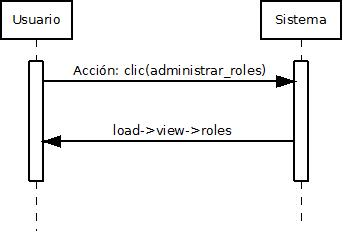
\includegraphics[width=0.6\textwidth]{ds_administrar_roles.jpg}
	\caption{Caso de uso: administrar roles.}
\end{figure}

\begin{figure}
	\centering
	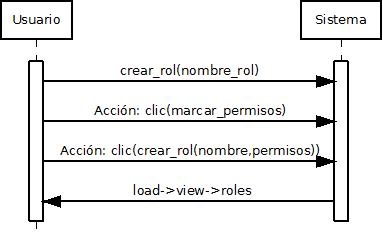
\includegraphics[width=0.6\textwidth]{ds_crear_rol.jpg}
	\caption{Caso de uso: crear rol.}
\end{figure}

\begin{figure}
	\centering
	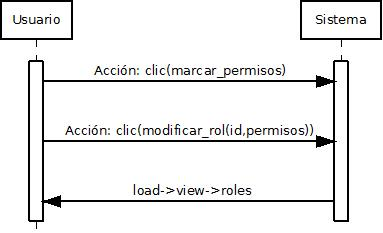
\includegraphics[width=0.6\textwidth]{ds_modificar_rol.jpg}
	\caption{Caso de uso: editar permisos de rol.}
\end{figure}

\begin{figure}
	\centering
	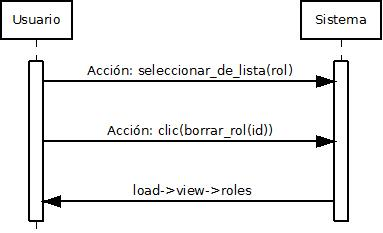
\includegraphics[width=0.6\textwidth]{ds_eliminar_rol.jpg}
	\caption{Caso de uso: eliminar rol.}
\end{figure}

\begin{figure}
	\centering
	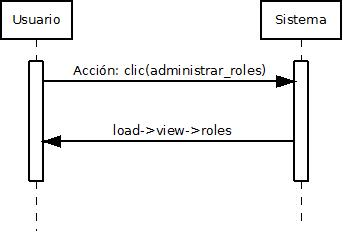
\includegraphics[width=0.6\textwidth]{ds_administrar_roles.jpg}
	\caption{Caso de uso: asignar rol.}
\end{figure}

\begin{figure}
	\centering
	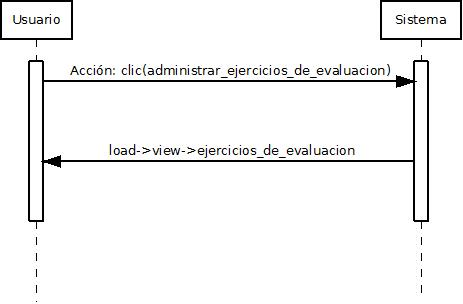
\includegraphics[width=0.6\textwidth]{ds_administrar_ejercicios_evaluacion.jpg}
	\caption{Caso de uso: administrar ejercicios de evaluación.}
\end{figure}

\begin{figure}
	\centering
	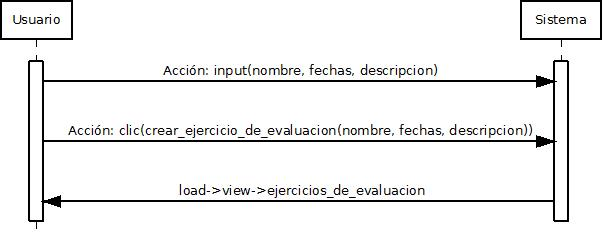
\includegraphics[width=0.6\textwidth]{ds_crear_ejercicio_evaluacion.jpg}
	\caption{Caso de uso: crear ejercicio de evaluación.}
\end{figure}

\begin{figure}
	\centering
	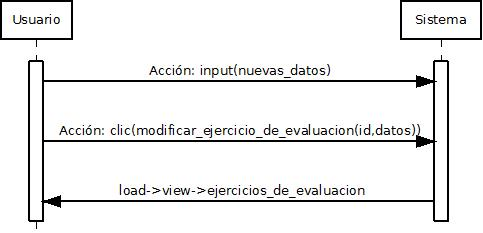
\includegraphics[width=0.6\textwidth]{ds_modificar_ejercicio_evaluacion.jpg}
	\caption{Caso de uso: editar ejercicio de evaluación.}
\end{figure}

\begin{figure}
	\centering
	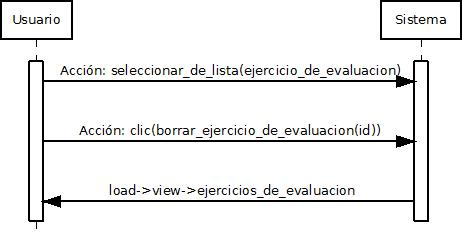
\includegraphics[width=0.6\textwidth]{ds_eliminar_ejercicio_evaluacion.jpg}
	\caption{Caso de uso: eliminar ejercicio de evaluación.}
\end{figure}

\begin{figure}
	\centering
	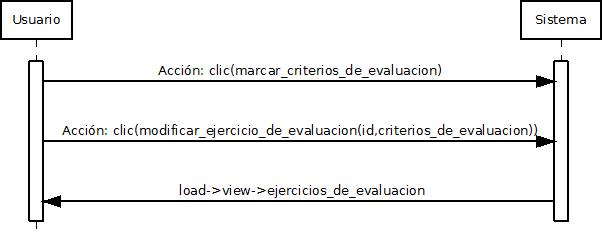
\includegraphics[width=0.6\textwidth]{ds_editar_criterios_de_evaluacion.jpg}
	\caption{Caso de uso: editar criterios de evaluación.}
\end{figure}

\begin{figure}
	\centering
	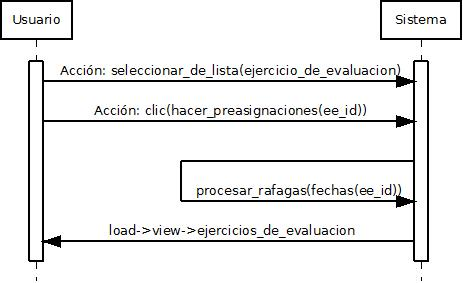
\includegraphics[width=0.6\textwidth]{ds_hacer_preasignaciones.jpg}
	\caption{Caso de uso: hacer preasignaciones.}
\end{figure}

\begin{figure}
	\centering
	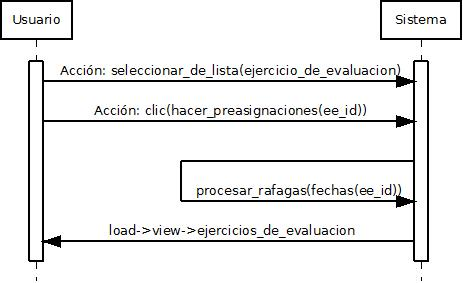
\includegraphics[width=0.6\textwidth]{ds_procesar_rafagas.jpg}
	\caption{Caso de uso: procesar ráfagas.}
\end{figure}

\begin{figure}
	\centering
	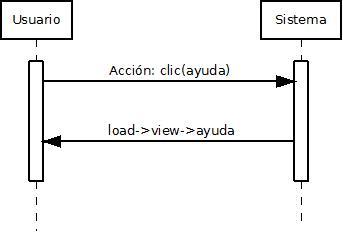
\includegraphics[width=0.6\textwidth]{ds_acceso_ayuda.jpg}
	\caption{Caso de uso: acceso a ayuda.}
\end{figure}

\newpage

\section{Modelo de Interfaz de Usuario}

En esta sección se detalla la navegación entre pantallas adjuntando imágenes de la interfaz del sistema, la principal forma de navegación es a través del menú superior.\\

A continuación se muestra la pantalla de inicio de sesión, en la cual es usuario debe introducir sus datos para acceder al sistema.\\

\begin{figure}[h!]
	\centering
	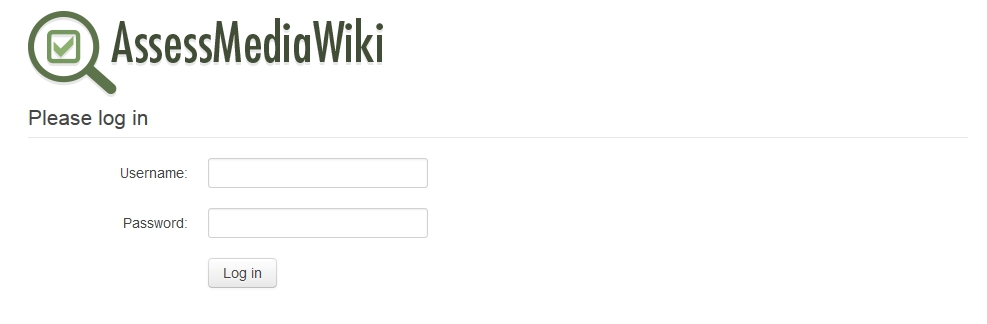
\includegraphics[width=0.9\textwidth]{sc_login.jpg}
	\caption{Pantalla de login.}
\end{figure}
\clearpage

Una vez iniciada sesión aparece la pantalla de inicio, donde aparecerán las evaluaciones disponibles para el usuario en casi de que hubiese, en cualquier momento podemos volver a esta pantalla haciendo clic en el botón "Assess" del menú superior.\\

\begin{figure}[h!]
	\centering
	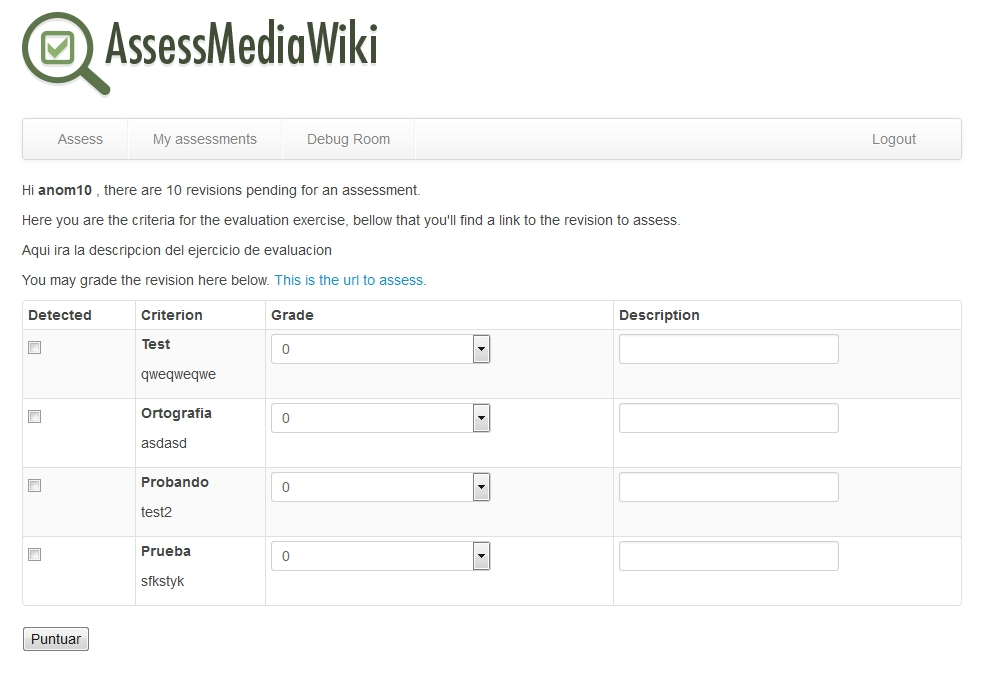
\includegraphics[width=0.9\textwidth]{sc_revision.jpg}
	\caption{Pantalla de inicio del usuario (sin la sala de debug, eso es debido a que el modo de desarrollo esta activado).}
\end{figure}
\clearpage

En caso de no haber evaluaciones disponibles para el usuario aparecerá el siguiente mensaje en la pagina principal.\\

\begin{figure}[h!]
	\centering
	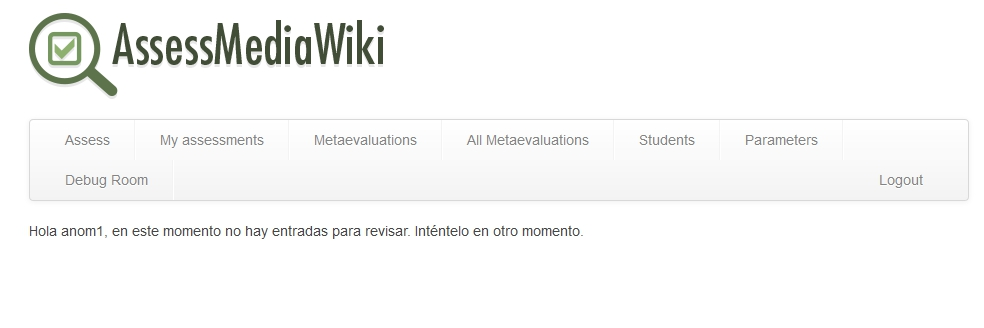
\includegraphics[width=0.9\textwidth]{sc_no_revision.jpg}
	\caption{Pantalla de usuario sin revisiones.}
\end{figure}
\clearpage

A partir de este punto usaremos capturas de pantalla con el perfil de profesor / administrador, ya que es el rol que tiene permisos para acceder a todas las secciones del sistema, los estudiantes tendrían los permisos básicos mostrados previamente.\\

A continuación se muestra la pantalla de metaevaluaciones, que estará disponible a trabes del botón "Metaevaluations" en el menú superior, para el profesor / administrador y para todos aquellos roles que el profesor / administrador lo haya habilitado.\\

\begin{figure}[h!]
	\centering
	\includegraphics[width=0.9\textwidth]{sc_metaevaluar.jpg}
	\caption{Pantalla de metaevaluaciones.}
\end{figure}
\clearpage

Si hacemos clic en el apartado del menú "All metaevaluations" podremos ver la lista completa de todas las metaevaluaciones realizadas existentes en el sistema, como podemos ver a continuacion.\\

\begin{figure}[h!]
	\centering
	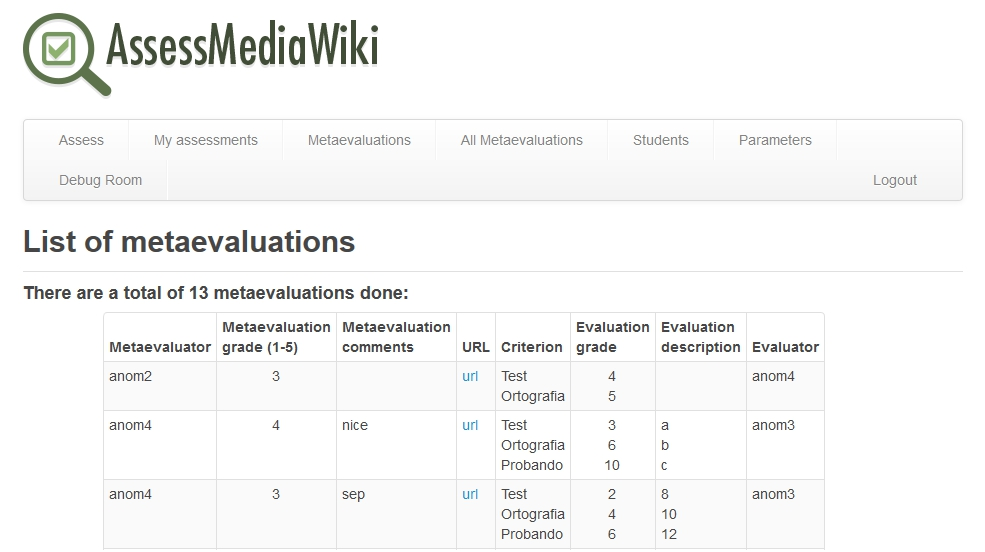
\includegraphics[width=0.9\textwidth]{sc_metaevaluar_lista.jpg}
	\caption{Pantalla de listado de metaevaluaciones.}
\end{figure}
\clearpage

Si hacemos clic en el apartado del menú "Students" podremos ver la lista completa de todos los estudiantes existentes en el sistema, y a través de los enlaces "Report", "Metaevaluations resume" y "CSV" podremos ver información detallada sobre las evaluaciones de los alumnos, las metaevaluaciones realizadas y generas un CSV (Coma Separated Values) respectivamente.\\

\begin{figure}[h!]
	\centering
	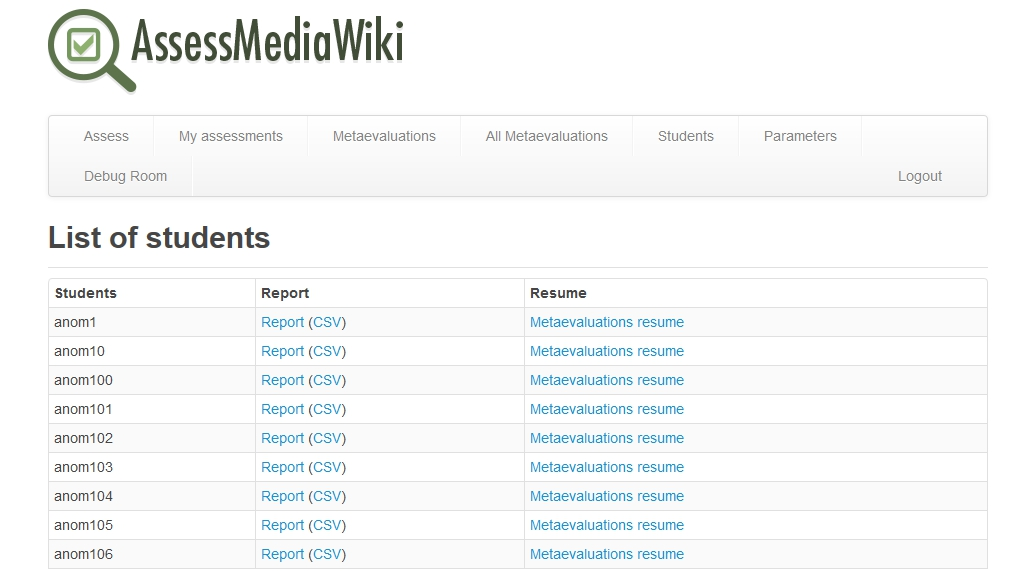
\includegraphics[width=0.9\textwidth]{sc_student_list.jpg}
	\caption{Pantalla de listado de alumnos.}
\end{figure}
\clearpage

Al hacer clic en el botón "Parameters" en el menú superior podremos acceder a configuraciones del sistema como vemos a continuacion.\\

Al final de la lista de parámetros encontraremos los botones "Administration of evaluation exercises", "Administration of roles" y "Help", funciones añadidas en esta nueva versión de AssessMediaWiki, cuyas interfaces veremos a continuacion.

\begin{figure}[h!]
	\centering
	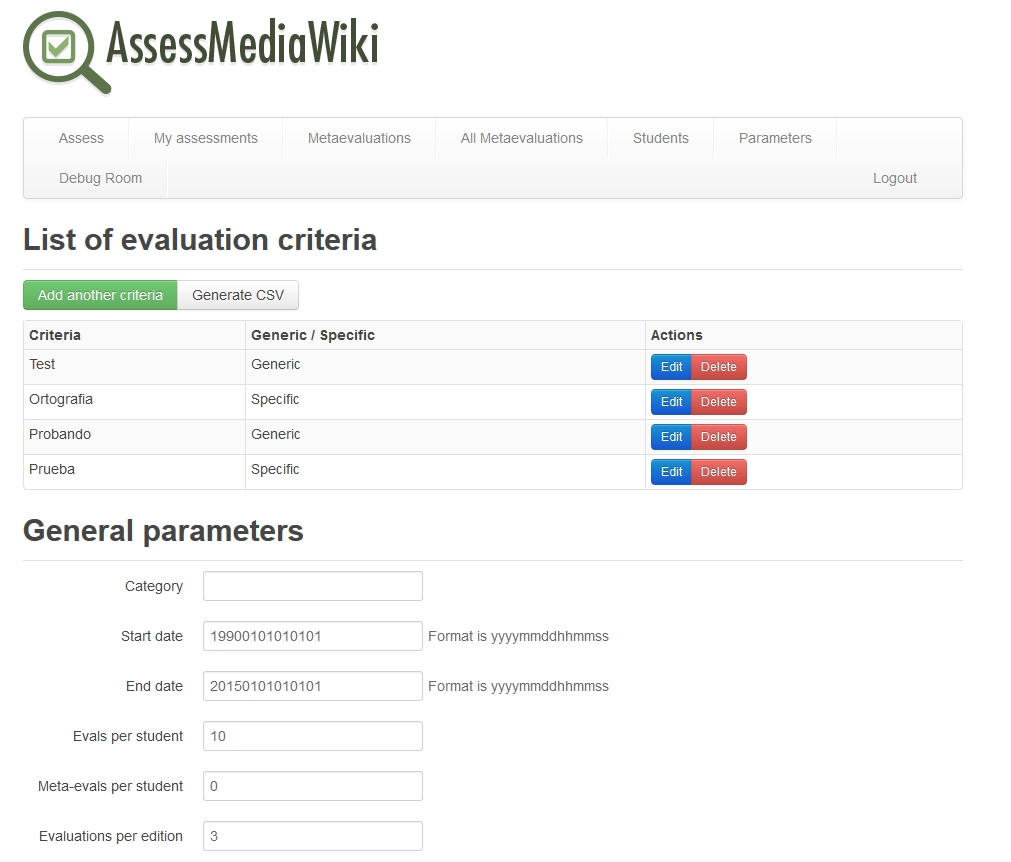
\includegraphics[width=0.9\textwidth]{sc_parametros1.jpg}
	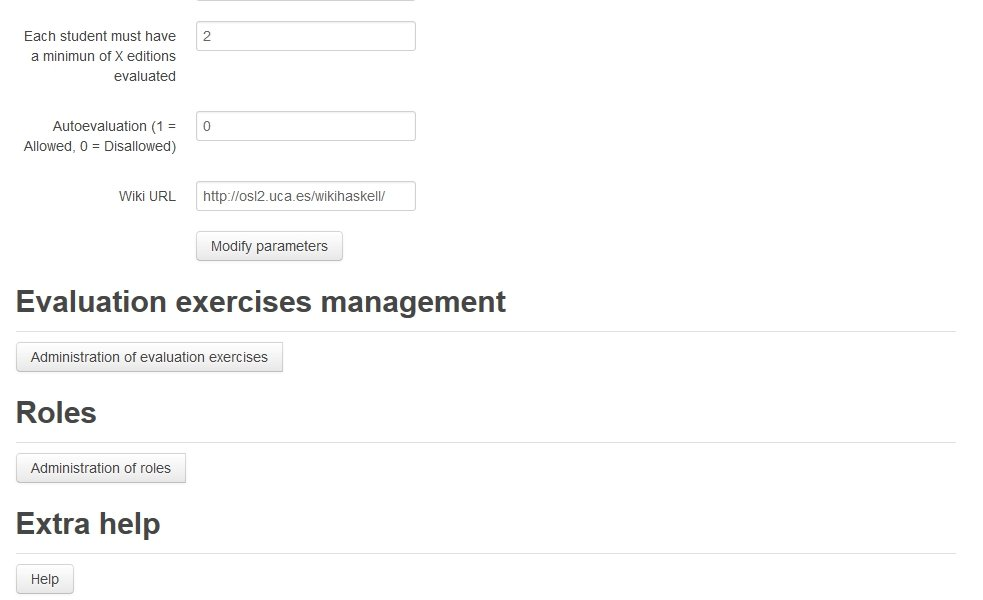
\includegraphics[width=0.9\textwidth]{sc_parametros2.jpg}
	\caption{Pantalla de parámetros.}
\end{figure}
\clearpage

A continuación veremos la interfaz de administración de roles, accesible desde el botón "Administration of roles" al final del listado de parámetros, a través de esta interfaz podremos crear nuevos roles, eliminar roles obsoletos, administrar los permisos de los roles existentes, asignar roles a los usuarios y ver que usuarios tienen roles asignados.\\

\begin{figure}[h!]
	\centering
	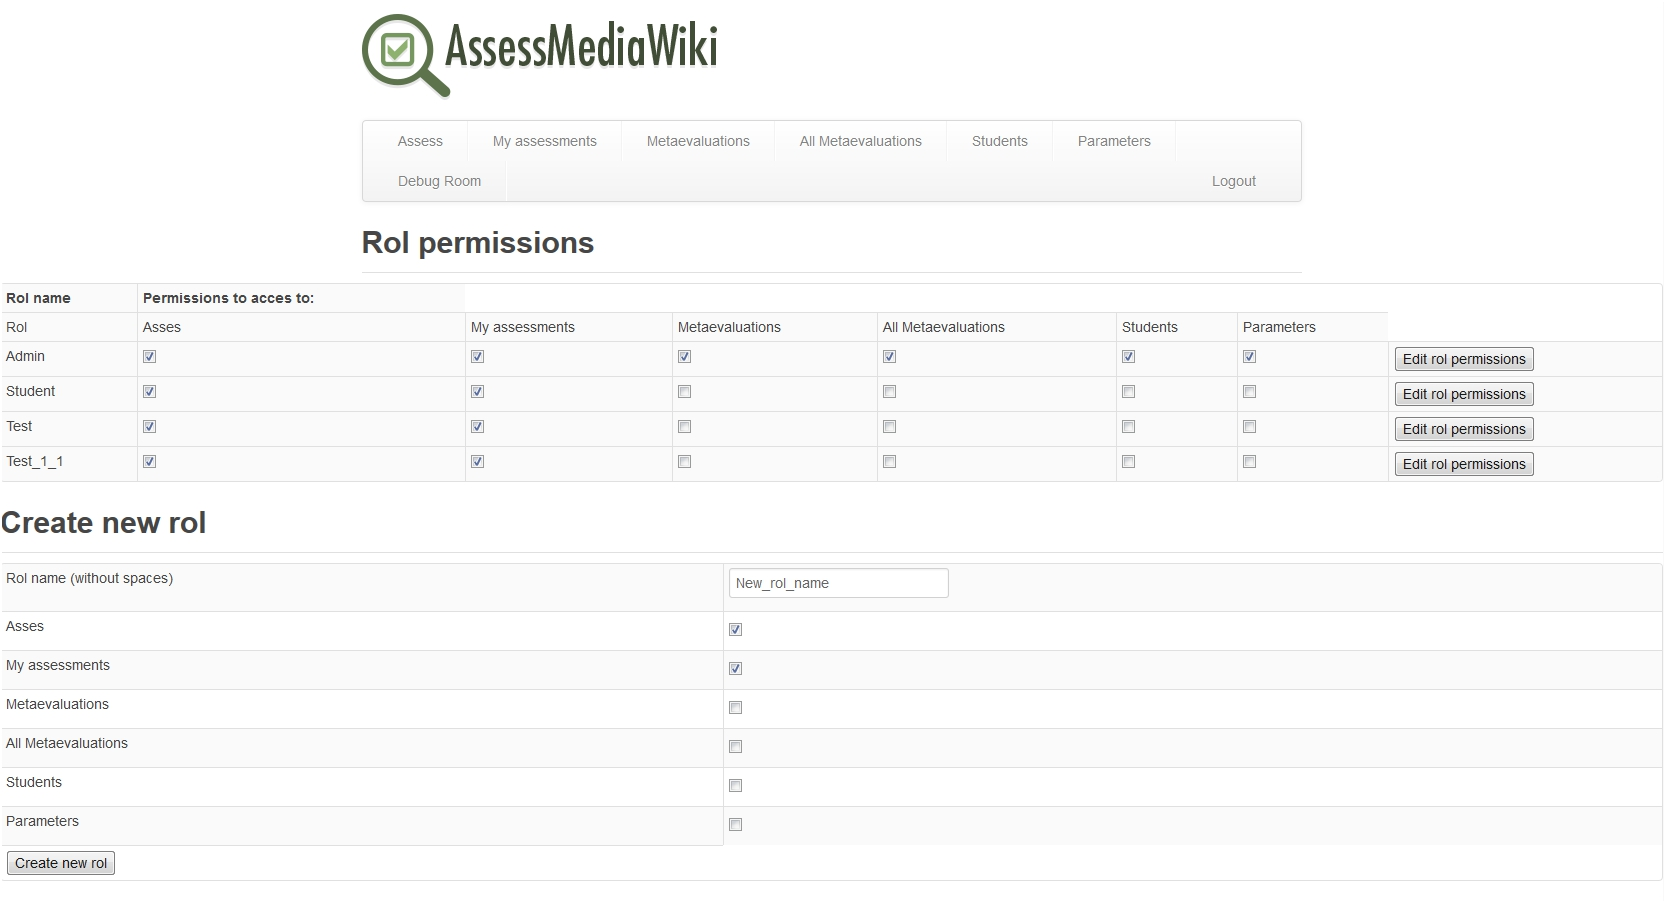
\includegraphics[width=0.9\textwidth]{sc_roles1.jpg}
	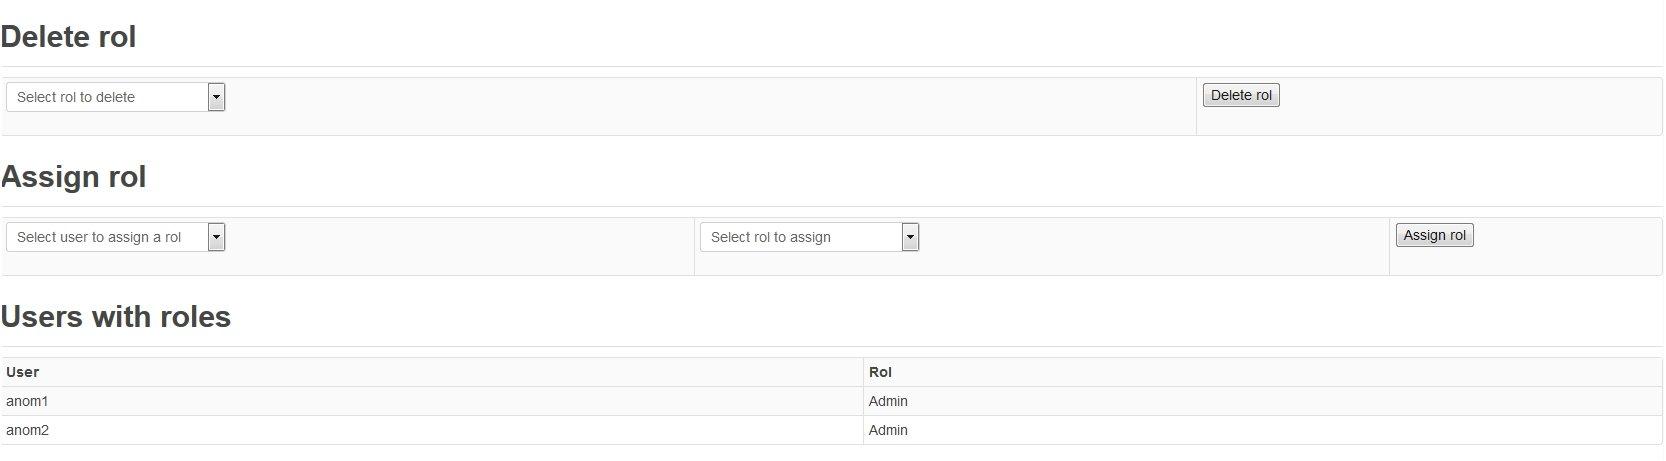
\includegraphics[width=0.9\textwidth]{sc_roles2.jpg}
	\caption{Pantalla de configuración de roles.}
\end{figure}
\clearpage

A continuación veremos la interfaz de administración de ejercicios de evaluación, accesible desde el botón "Administration of evaluation exercises" al final del listado de parámetros, a través de esta interfaz podremos crear nuevos ejercicios de evaluación, eliminar ejercicios de evaluación, administrar los parámetros de los ejercicios de evaluación existentes, modificar las categorías a evaluar en los ejercicios de evaluación correspondientes.\\

\begin{figure}[h!]
	\centering
	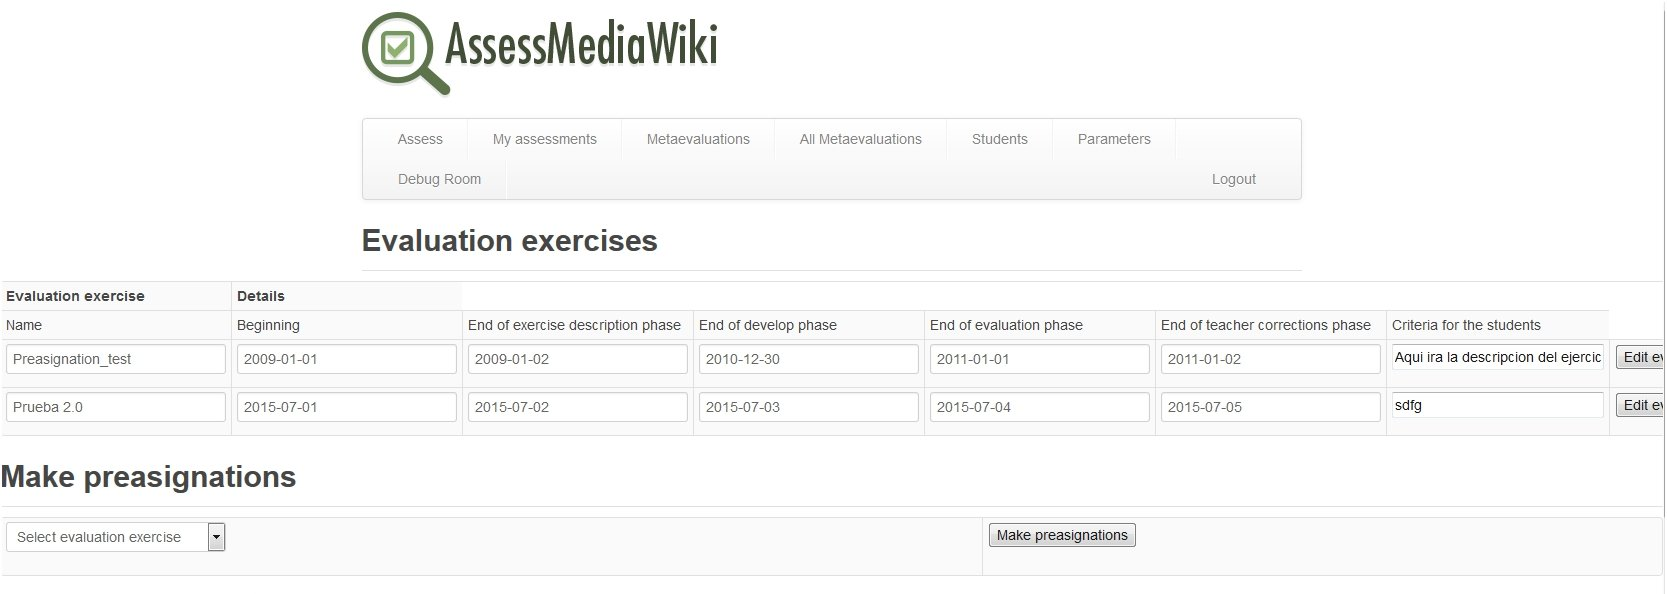
\includegraphics[width=0.9\textwidth]{sc_ee1.jpg}
	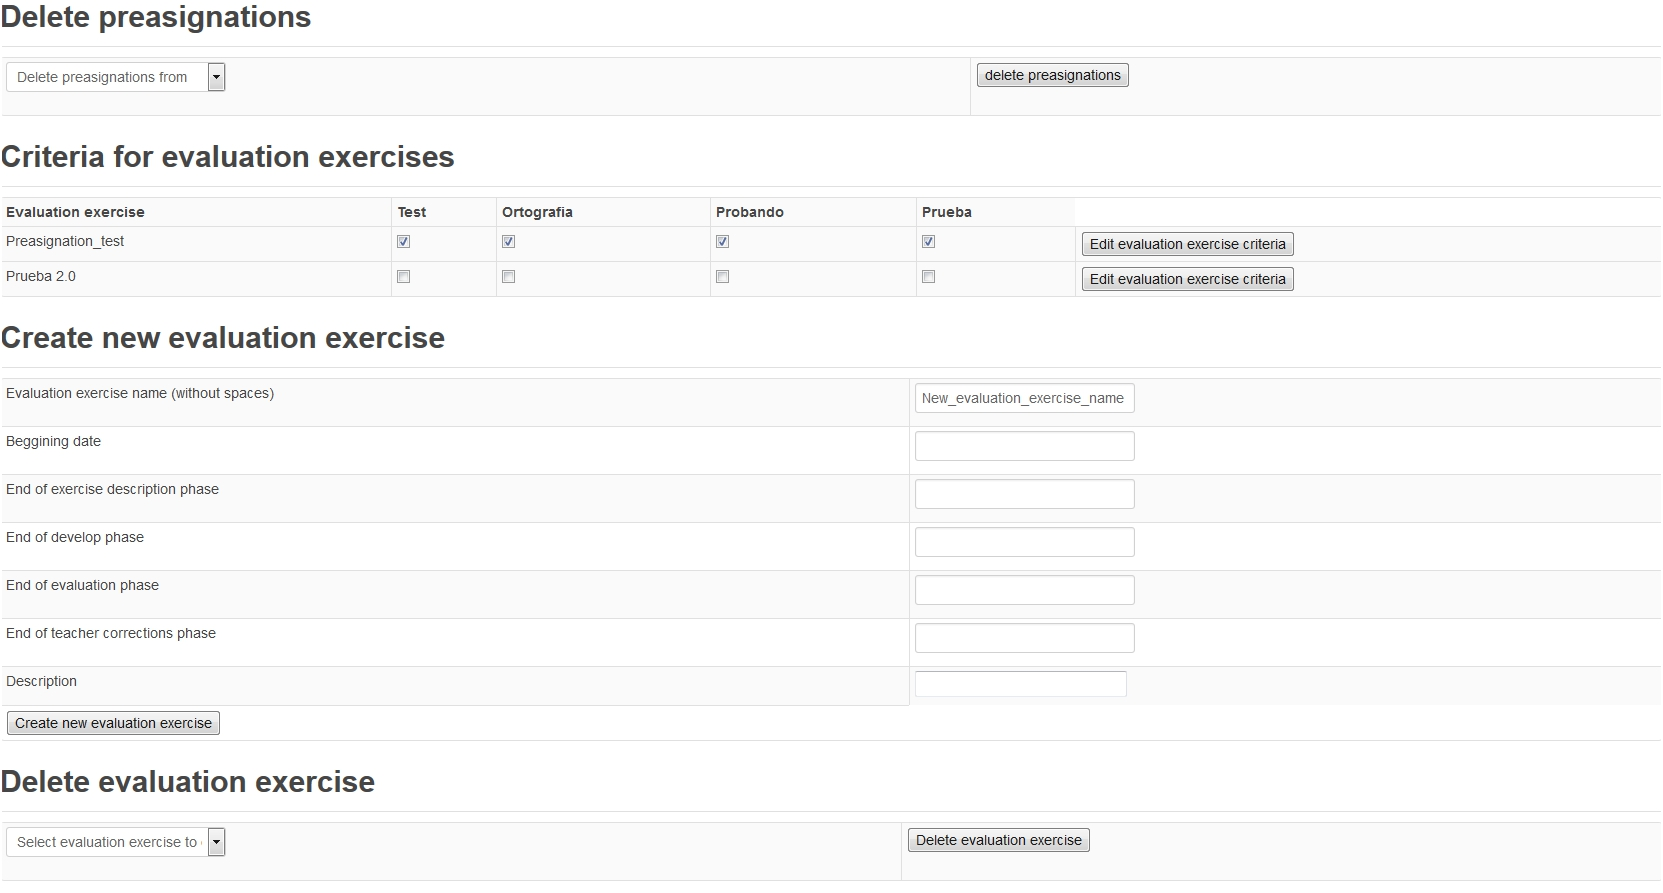
\includegraphics[width=0.9\textwidth]{sc_ee2.jpg}
	\caption{Pantalla de configuración de ejercicios de evaluación.}
\end{figure}
\clearpage

A continuación veremos la interfaz de ayuda extra, accesible desde el botón "Help" al final del listado de parámetros,  en esta nueva interfaz se mostrara información al usuario en caso de que necesite recordar el uso de alguna característica del sistema.\\

\begin{figure}[h!]
	\centering
	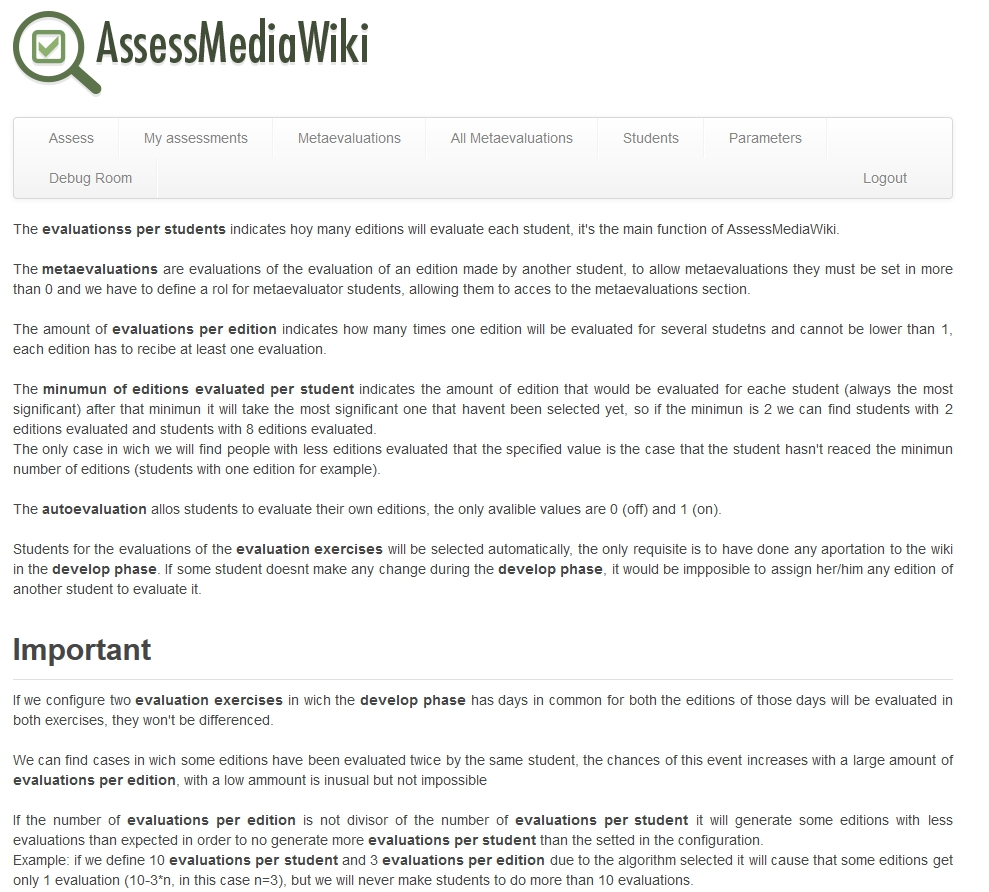
\includegraphics[width=0.9\textwidth]{sc_extra_help.jpg}
	\caption{Pantalla de ayuda extra.}
\end{figure}
\clearpage

\chapter{Diseño del Sistema}
% ------------------------------------------------------------------------------
% Este fichero es parte de la plantilla LaTeX para la realización de Proyectos
% Final de Grado, protegido bajo los términos de la licencia GFDL.
% Para más información, la licencia completa viene incluida en el
% fichero fdl-1.3.tex

% Copyright (C) 2012 SPI-FM. Universidad de Cádiz
% ------------------------------------------------------------------------------

\section{Arquitectura del Sistema}
La estructura del sistema esta basada en el esquema de modelo vista controlador, introducidos en \href{http://www.codeigniter.com/}{CodeIgniter} ademas de una base de datos propia y la base de datos del media wiki, de forma que encontraremos los archivos principales en las carpetas de vista, donde se genera la interfaz para el usuario, modelo, donde se encuentran las funciones y algoritmo para el funcionamiento interno, y controladores, donde hacemos que se comuniquen las vistas con los modelos.

\subsection{Arquitectura Física}
Son necesarios para nuestro sistema un ordenador que actué de servidor (puede valer donde este montado el Media Wiki) y el ordenador propio de los usuarios, con los cuales interactuaran con el sistema.

En principio AssessMediaWiki esta pensado para ser independiente del sistema operativo, decisión que verse afectada en un futuro dependiendo de las necesidades de escalabilidad y las funciones que se quieran implementar.

\subsection{Arquitectura Lógica}
La arquitectura del sistema se divide en las siguientes capas

\paragraph*{Modelo}
En este grupo podemos encontrar todo el software que genera las funciones para obtener, generar datos e interactuar con las bases de datos.

\paragraph*{Vista}
En este grupo podemos encontrar todo el software que genera la interfaz del usuario, siendo esta su funcionalidad exclusiva.

\paragraph*{Controlador}
Aquí encontraremos el software que completa los campos de las vistas, comunicándolas con los modelos. Los controladores se encargan de mostrar los datos del sistema en las vistas, e interaccionar con los usuarios, ya sea modificando dichos datos o navegando entre las distintas vistas.

\paragraph*{Bases de datos}
Nuestro sistema cuenta con dos bases de datos fundamentales, la base de datos del MediaWiki, donde se guarda toda la información de los alumnos y su aportación al Wiki, y la base de datos del AssessMediaWiki, donde almacenaremos la nueva información generada por la interacción de los usuarios.

\begin{figure}[h!]
	\centering
	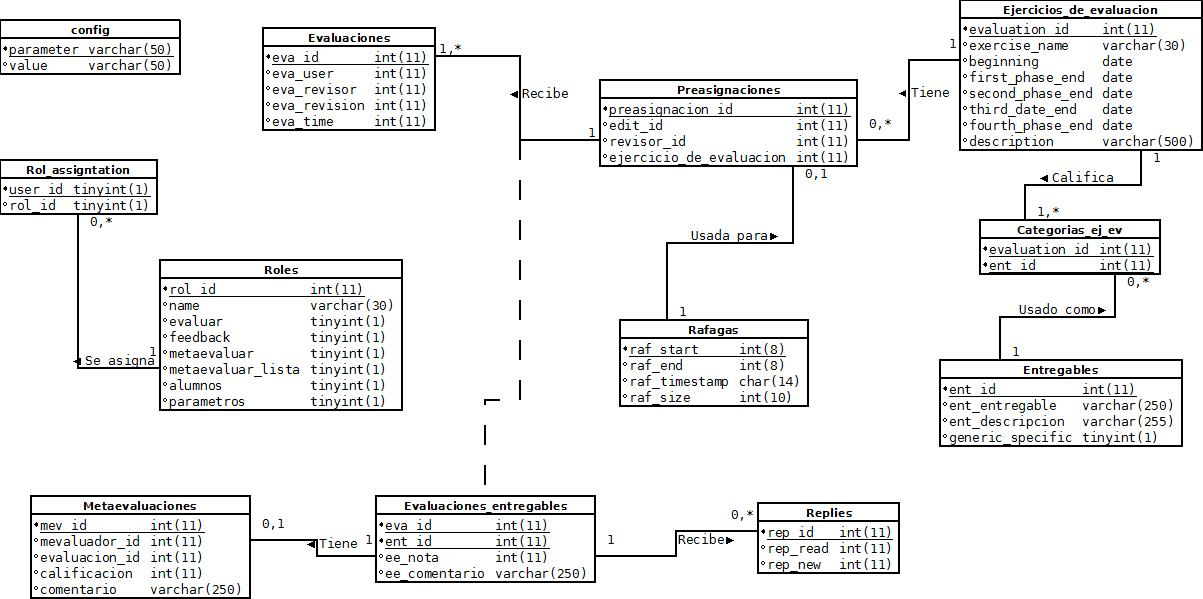
\includegraphics[width=0.9\textwidth]{db2.jpg}
	\caption{Diagrama de la base de datos de AMW 2.0.}
\end{figure}

\begin{figure}[h!]
	\centering
	\includegraphics[width=0.9\textwidth]{mediawikidb.png}
	\caption{Diagrama de la base de datos de MediaWiki (disponible en la web de MediaWiki).}
\end{figure}

\newpage

\section{Parametrización del software base}
Sera necesario editar el archivo de configuración para introducir los datos de nuestro MediaWiki, permitiendo así acceso a la base de datos y a generar las URLs para las evaluaciones (este proceso se explica detalladamente en el manual de instalación). También tenemos la opción de activar o desactivar el modo de desarrollo para hacer pruebas o cambios según se requiera.

\section{Diseño Físico de Datos}
En esta sección se define la estructura física de datos que utilizará el sistema, a partir del modelo de conceptual de clases, de manera que teniendo presente los requisitos establecidos para el sistema de información y las particularidades del entorno tecnológico, se consiga un acceso eficiente de los datos.
La estructura física se compone de tablas, índices, procedimientos almacenados, secuencias y otros elementos dependientes del SGBD a utilizar.

\begin{figure}[!h]
	\centering
	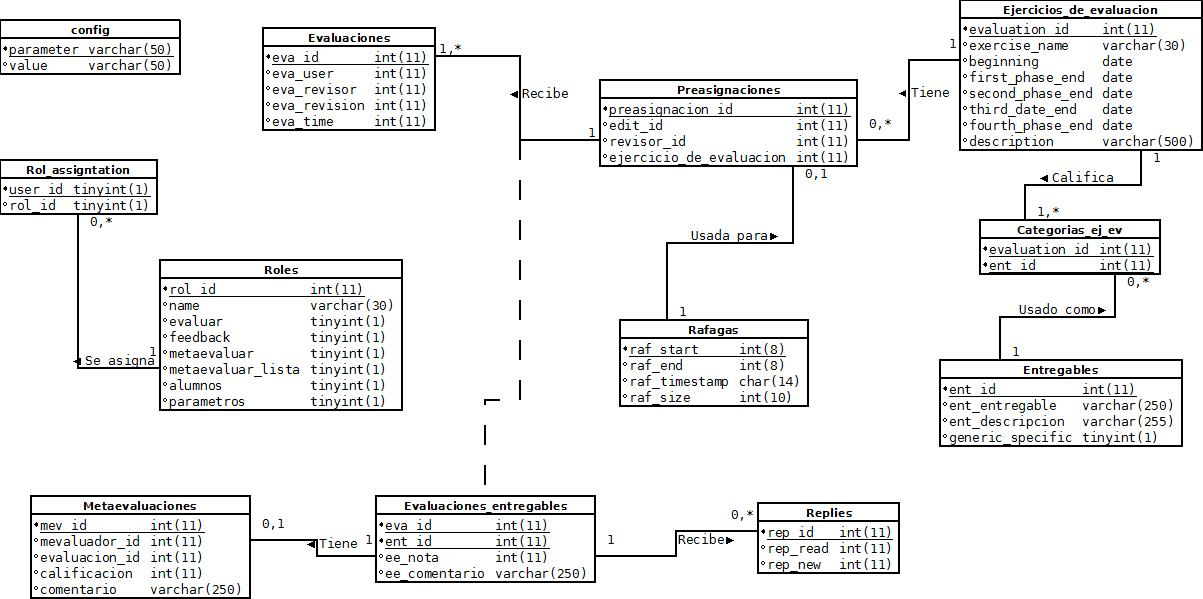
\includegraphics[width=0.9\textwidth]{db2.jpg}
	\caption{Diagrama de la base de datos de AMW 2.0.}
\end{figure}




\chapter{Construcción del Sistema}
% ------------------------------------------------------------------------------
% Este fichero es parte de la plantilla LaTeX para la realización de Proyectos
% Final de Grado, protegido bajo los términos de la licencia GFDL.
% Para más información, la licencia completa viene incluida en el
% fichero fdl-1.3.tex

% Copyright (C) 2012 SPI-FM. Universidad de Cádiz
% ------------------------------------------------------------------------------

Este capítulo trata sobre todos los aspectos relacionados con la implementación del sistema en código, haciendo uso de un determinado entorno tecnológico.

\section{Entorno de Construcción}
En esta sección se debe indicar el marco tecnológico utilizado para la construcción del sistema: entorno de desarrollo (IDE), lenguaje de programación, herramientas de ayuda a la construcción y despliegue, control de versiones, repositorio de componentes, integración contínua, etc.

Para desarrollar este proyecto hemos usado:

\begin{itemize}
	\item \href{http://www.codeigniter.com/}{CodeIgniter} [\url{http://www.codeigniter.com/}]
	\item \href{https://secure.php.net/}{PHP} [\url{https://secure.php.net/}]
	\item HTML[\url{https://es.wikipedia.org/wiki/HTML}]
	\item \href{https://www.mysql.com/}{MYSQL} [\url{https://www.mysql.com/}]
	\item \href{https://forja.rediris.es/}{Forja Rediris} [\url{https://forja.rediris.es/}]
	\item \href{http://tortoisesvn.net/}{Tortoise SVN} [\url{http://tortoisesvn.net//}]
	\item \href{https://www.mozilla.org/es-ES/}{Firefox} [\url{https://www.mozilla.org/es-ES/}]
	\item \href{http://www.latex-project.org/}{LaTeX} [\url{http://www.latex-project.org/}]
	\item \href{http://www.texstudio.org/}{TeXtudio} [\url{http://www.texstudio.org/}]
	\item \href{http://dia-installer.de/index.html.es}{Dia} [\url{http://dia-installer.de/index.html.es}]	
\end{itemize}

\section{Código Fuente}
Organización del código fuente, describiendo la utilidad de los diferentes ficheros y su distribución en paquetes o directorios. Asimismo, se incluirá algún extracto significativo de código fuente que sea de interés para ilustrar algún algoritmo o funcionalidad específica del sistema.\\

Se ha usado una estructura modelo vista controlador, de forma que al analizar inicialmente el sistema, pude ver que en la carpeta de vista guardaremos las interfaces, en la de modelos guardaremos los objetos donde se definen todas las funciones y en la carpeta de controladores guardaremos los controladores, que hacen posible que vistas y modelos interactúen entre si.\\

También me gustaría destacar el algoritmo de barajado aleatorio usado para la preasignación de ediciones a los alumnos.\\
Fuente: 
\href{https://es.wikipedia.org/wiki/Algoritmo_Fisher-Yates}{Wikipedia: Algoritmo Fisher-Yates}

Otra cosa a destacar es que con el antiguo esquema de la base de datos, al realizarse una re-evaluación, esta no era tratada de forma especial, y contaba como si fuese una evaluación normal de una edición.
Gracias a la nueva distribución de la base de datos se ha solventado ese problema, manteniendo a su vez la compatibilidad con otros sistemas como StatMediaWiki o CleverFigures

\section{Scripts de Base de datos}
El script para la creación de la base de datos, así como para introducir los datos y valores iniciales es el siguiente:\\

-- --------------------------------------------------------\\

--\\
-- Estructura de tabla para la tabla `config`\\
--\\

CREATE TABLE IF NOT EXISTS `config` (\\
`parameter` varchar(50) NOT NULL,\\
`value` varchar(50) NOT NULL,\\
PRIMARY KEY (`parameter`)\\
) ENGINE=InnoDB DEFAULT CHARSET=utf8;\\

-- --------------------------------------------------------\\

--\\
-- Estructura de tabla para la tabla `entregables`\\
--\\

CREATE TABLE IF NOT EXISTS `entregables` (\\
`ent\_id` int(11) NOT NULL AUTO\_INCREMENT,\\
`ent\_entregable` varchar(250) NOT NULL,\\
`ent\_description` varchar(255) NOT NULL,\\
`generic\_specific` boolean NOT NULL DEFAULT false, --0 = generic, 1 = specific\\
PRIMARY KEY (`ent\_id`)\\
) ENGINE=InnoDB  DEFAULT CHARSET=utf8 AUTO\_INCREMENT=1 ;\\

-- --------------------------------------------------------\\

--\\
-- Estructura de tabla para la tabla `evaluaciones`\\
--\\

CREATE TABLE IF NOT EXISTS `evaluaciones` (\\
`eva\_id` int(11) NOT NULL AUTO\_INCREMENT,\\
`eva\_user` int(11) NOT NULL,\\
`eva\_revisor` int(11) NOT NULL,\\
`eva\_revision` int(11) NOT NULL,\\
`eva\_time` int(11) NOT NULL,\\
PRIMARY KEY (`eva\_id`)\\
) ENGINE=InnoDB  DEFAULT CHARSET=utf8 AUTO\_INCREMENT=1 ;\\

-- --------------------------------------------------------\\

--\\
-- Estructura de tabla para la tabla `evaluaciones\_entregables`\\
--\\

CREATE TABLE IF NOT EXISTS `evaluaciones\_entregables` (\\
`eva\_id` int(11) NOT NULL,\\
`ent\_id` int(11) NOT NULL,\\
`ee\_nota` int(11) NOT NULL,\\
`ee\_comentario` varchar(250) NOT NULL,\\
PRIMARY KEY (`eva\_id`,`ent\_id`)\\
) ENGINE=InnoDB DEFAULT CHARSET=utf8;\\

-- --------------------------------------------------------\\

--\\
-- Estructura de tabla para la tabla `replies`\\
--\\

CREATE TABLE IF NOT EXISTS `replies` (\\
`rep\_id` int(11) NOT NULL AUTO\_INCREMENT,\\
`rep\_read` int(11) NOT NULL,\\
`rep\_new` int(11) NOT NULL,\\
PRIMARY KEY (`rep\_id`)\\
) ENGINE=InnoDB  DEFAULT CHARSET=utf8 AUTO\_INCREMENT=1 ;\\

-- --------------------------------------------------------\\

--\\
-- Estructura de tabla para la tabla `metaevaluaciones`\\
--\\

CREATE TABLE IF NOT EXISTS `metaevaluaciones` (\\
`mev\_id` int(11) NOT NULL AUTO\_INCREMENT,\\
`mevaluador\_id` int(11) NOT NULL,\\
`evaluacion\_id` int(11) NOT NULL,\\
`calificacion` int(11) NOT NULL,\\
`comentario` varchar(250) NOT NULL,\\
PRIMARY KEY (`mev\_id`)\\
) ENGINE=InnoDB  DEFAULT CHARSET=utf8 AUTO\_INCREMENT=1 ;\\

-- --------------------------------------------------------\\

--\\
-- Estructura de tabla para la tabla `roles`\\
--\\

CREATE TABLE IF NOT EXISTS `roles` (\\
`rol\_id` int(11) NOT NULL AUTO\_INCREMENT,\\
`name` varchar(30) NOT NULL UNIQUE,\\
`evaluar` boolean NOT NULL DEFAULT true,\\
`feedback` boolean NOT NULL DEFAULT true,\\
`metaevaluar` boolean NOT NULL DEFAULT false,\\
`metaevaluar\_lista` boolean NOT NULL DEFAULT false,\\
`alumnos` boolean NOT NULL DEFAULT false,\\
`parametros` boolean NOT NULL DEFAULT false,\\
PRIMARY KEY (`rol\_id`)\\
) ENGINE=InnoDB  DEFAULT CHARSET=utf8 AUTO\_INCREMENT=1 ;\\

-- --------------------------------------------------------\\

--\\
-- Estructura de tabla para la tabla `rol\_assignation`\\
--\\

CREATE TABLE IF NOT EXISTS `rol\_assignation` (\\
`user\_id` int(11) NOT NULL,\\
`rol\_id` int(11) NOT NULL,\\
PRIMARY KEY (`user\_id`)\\
) ENGINE=InnoDB DEFAULT CHARSET=utf8 AUTO\_INCREMENT=1 ;\\

-- --------------------------------------------------------\\

--\\
-- Estructura de tabla para la tabla `ejercicios\_de\_evaluacion`\\
--\\

CREATE TABLE IF NOT EXISTS `ejercicios\_de\_evaluacion` (\\
`evaluation\_id` int(11) NOT NULL AUTO\_INCREMENT,\\
`exercise\_name` varchar(30) NOT NULL UNIQUE,\\
`beginning` date NOT NULL,\\
`first\_phase\_end` date NOT NULL,\\
`second\_phase\_end` date NOT NULL,\\
`third\_phase\_end` date NOT NULL,\\
`fourth\_phase\_end` date NOT NULL,\\
`description` varchar(500) NOT NULL,\\
PRIMARY KEY (`evaluation\_id`)\\
) ENGINE=InnoDB DEFAULT CHARSET=utf8 AUTO\_INCREMENT=1 ;\\

-- ----------------------------------------------------------\\

--\\
-- Estructura de tabla para la tabla `preasignaciones`\\
--\\

CREATE TABLE IF NOT EXISTS `preasignaciones` (\\
`preasignacion\_id` int(11) NOT NULL AUTO\_INCREMENT,\\
`edit\_id` int(11) NOT NULL,\\
`revisor\_id` int(11) NOT NULL,\\
`ejercicio\_de\_evaluacion` int(11) NOT NULL,\\
PRIMARY KEY (`preasignacion\_id`)\\
) ENGINE=InnoDB DEFAULT CHARSET=utf8 AUTO\_INCREMENT=1 ;\\

-- --------------------------------------------------------\\

--\\
-- Estructura de tabla para la tabla `categorias\_ej\_ev`\\
--\\

CREATE TABLE IF NOT EXISTS `categorias\_ej\_ev` (\\
`evaluation\_id` int(11) NOT NULL,\\
`ent\_id` int(11) NOT NULL,\\
PRIMARY KEY (`evaluation\_id`,`ent\_id`)\\
) ENGINE=InnoDB DEFAULT CHARSET=utf8 AUTO\_INCREMENT=1 ;\\

-- --------------------------------------------------------\\

--\\
-- Estructura de tabla para la tabla `rafagas`\\
--\\

CREATE TABLE IF NOT EXISTS `rafagas` (\\
`raf\_start` int(8) NOT NULL,\\
`raf\_end` int(8) NOT NULL,\\
`raf\_timestamp` char(14) NOT NULL,\\
`raf\_size` int(10) NOT NULL,\\
PRIMARY KEY (`raf\_start`)\\
) ENGINE=InnoDB DEFAULT CHARSET=utf8;\\

-- --------------------------------------------------------\\


--\\
-- Insercion de valores por defecto\\
--
-- A la vez que creamos la tabla añadimos los dos primeros usuarios, esto ha de hacerse como ultima accion\\
-- ya que si esta creado dara error y no se crearan las siguientes tablas, y una vez añadidos los usuarios\\
-- añadimos al primer usuario creado en la wiki como administrador.\\
-- \#TODO evitar esse error

INSERT INTO `roles`(`name`, `evaluar`, `feedback`, `metaevaluar`, `metaevaluar\_lista`, `alumnos`,\\ `parametros`)\\
VALUES ("Admin",1,1,1,1,1,1);\\
INSERT INTO `roles`(`name`, `evaluar`, `feedback`)  \\
VALUES ("Student",1,1);\\
INSERT INTO `rol\_assignation`(`user\_id`, `rol\_id`)\\
VALUES (1,1);\\

-- --------------------------------------------------------\\


La mayoría de funciones para manejar las bases de datos se encuentran en los modelos del sistema.\\

Como se ha mencionado anteriormente, al modificar la estructura de la base de datos del sistema (ver [Fig.6.1] y [Fig.6.2] a continuación) se ha conseguido solventar algunas debilidades de la versión anterior, así como implementar mejoras como las ráfagas y las preasignaciones, para las cuales es necesario que las bases de datos de AssessMediaWiki y MediaWiki se intercomuniquen, ese proceso se puede observar con mas detenimiento en el modelo de ejercicios de evaluación.

\clearpage

\begin{figure}
	\centering
	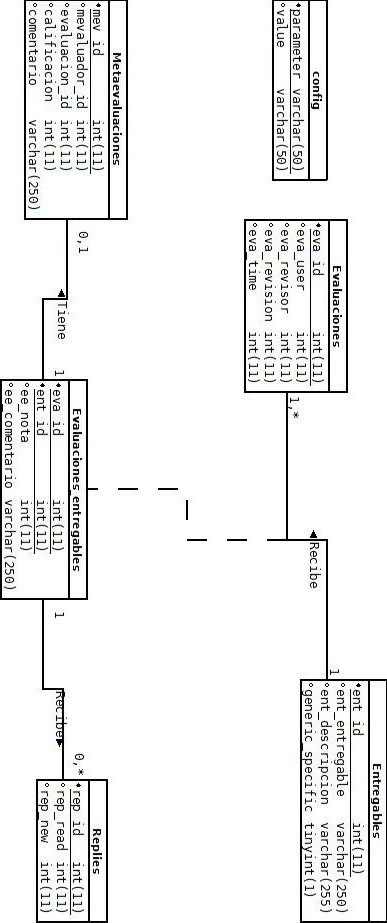
\includegraphics[width=0.6\textwidth]{db1girada.jpg}
	\caption{Diagrama de la base de datos de AMW 1.0.}
\end{figure}

\begin{figure}
	\centering
	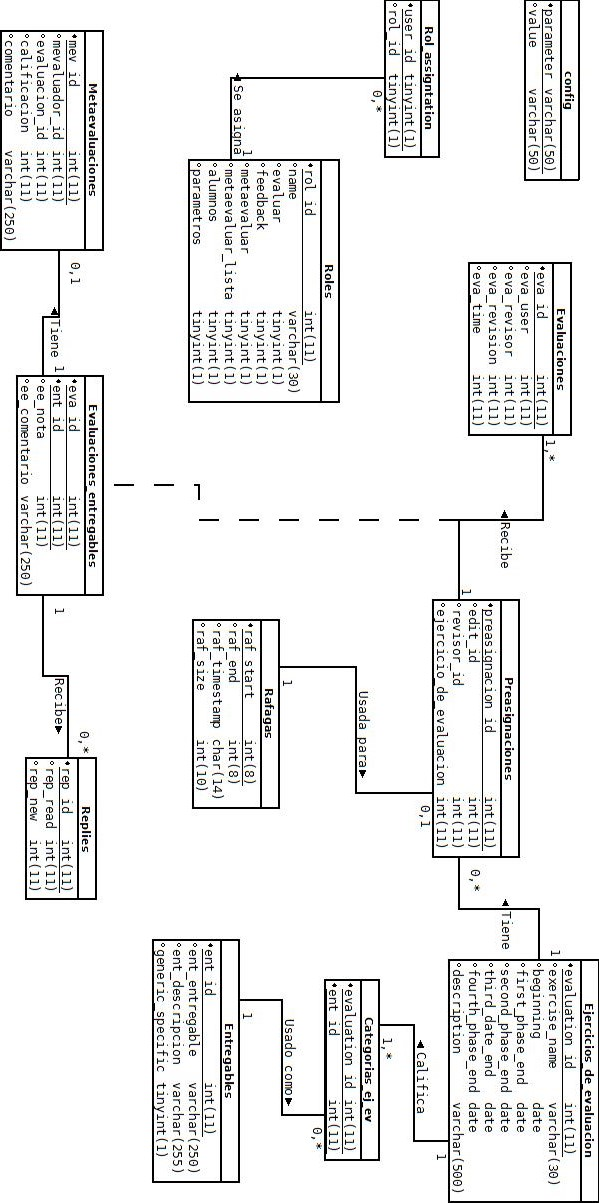
\includegraphics[width=0.6\textwidth]{db2girada.jpg}
	\caption{Diagrama de la base de datos de AMW 2.0.}
\end{figure}

\clearpage

\chapter{Pruebas del Sistema}
% ------------------------------------------------------------------------------
% Este fichero es parte de la plantilla LaTeX para la realización de Proyectos
% Final de Grado, protegido bajo los términos de la licencia GFDL.
% Para más información, la licencia completa viene incluida en el
% fichero fdl-1.3.tex

% Copyright (C) 2012 SPI-FM. Universidad de Cádiz
% ------------------------------------------------------------------------------

En este capítulo se presenta el plan de pruebas del sistema de información, incluyendo los diferentes tipos de pruebas que se han llevado a cabo, ya sean manuales (mediante listas de comprobación) o automatizadas mediante algún software específico de pruebas.

\section{Estrategia}
En esta sección se debe incluir el alcance de las pruebas, hasta donde se pretende llegar con ellas, si se registrarán todas o sólo aquellas de un cierto tipo y cómo se interpretarán y evaluarán los resultados.
También, se incluirá el procedimiento a seguir para las pruebas de regresión, esto es, la repetición de ciertas pruebas para comprobar que nuevos cambios que se vayan introduciendo no originen errores en el software ya probado.

\section{Entorno de Pruebas}
Incluir en este apartado los requisitos de los entornos hardware/software donde se ejecutarán las pruebas.

\section{Roles}
Describir en esa sección cuáles serán los perfiles y participantes necesarios para la ejecución de cada uno de los niveles de prueba.

\section{Niveles de Pruebas}
En este sección se documentan los diferentes tipos de pruebas que se han llevado a cabo, ya sean manuales o automatizadas mediante algún software específico de pruebas.

\subsection{Pruebas Unitarias}
Las pruebas unitarias tienen por objetivo localizar errores en cada nuevo artefacto software desarrollado, antes que se produzca la integración con el resto de artefactos del sistema.

\subsection{Pruebas de Integración}
Este tipo de pruebas tienen por objetivo localizar errores en módulos o subsistemas completos, analizando la interacción entre varios artefactos software.

\subsection{Pruebas de Sistema}
En esta actividad se realizan las pruebas de sistema de modo que se asegure que el sistema cumple con todos los requisitos establecidos: funcionales, de almacenamiento, reglas de negocio y no funcionales. Se suelen desarrollar en un entorno específico para pruebas.

\subsubsection{Pruebas Funcionales}
Con estas pruebas se analiza el buen funcionamiento de la implementación de los flujos normales y alternativos de los distintos casos de uso del sistema.

\subsubsection{Pruebas No Funcionales}
Estas pruebas pretenden comprobar el funcionamiento del sistema, con respecto a los requisitos no funcionales identificados: eficiencia, seguridad, etc.

\subsection{Pruebas de Aceptación}
El objetivo de estas pruebas es demostrar que el producto está listo para el paso a producción. Suelen ser las mismas pruebas que se realizaron anteriormente pero en el entorno de producción. En estas pruebas, es importante la participación del cliente final.

% EPILOGO
\part{Epílogo}
\null\vfill
\noindent En esta última parte quedarán recogidas las conclusiones y los manuales necesarios para el manejo de la aplicación resultado del desarrollo. Si se ha realizado algún tipo de evaluación de la solución proporcionada, más allá de las pruebas del sistema, también deberá venir recogida en un capítulo separado dentro de esta parte. Pueden consultarse diversos tipos de evaluaciones sobre sistemas de información en \cite{hevner2004}: casos de estudio, análisis estático, análisis dinámico, simulación, experimento controlado, etc.
\vfill

\chapter{Manual de implantación y explotación}
% ------------------------------------------------------------------------------
% Este fichero es parte de la plantilla LaTeX para la realización de Proyectos
% Final de Grado, protegido bajo los términos de la licencia GFDL.
% Para más información, la licencia completa viene incluida en el
% fichero fdl-1.3.tex

% Copyright (C) 2012 SPI-FM. Universidad de Cádiz
% ------------------------------------------------------------------------------

Las instrucciones de instalación y explotación del sistema se detallan a continuación.

\section{Introducción}
AssessMediaWiki es una aplicación web de código abierto que, al conectarse a una instalación MediaWiki, proporciona procedimientos de autoevaluación, hetero evaluación y evaluación entre iguales, a la vez que mantiene información sobre esas evaluaciones. Los supervisores pueden obtener informes que ayudan en la evaluación de los estudiantes.
\newline

Aunque hay un gran número de extensiones para el sistema MediaWiki, no hemos encontrado ninguna que permitiera evaluar contribuciones individuales a un wiki. La mayoría de las aproximaciones solo ofrecen formas de evaluar una versión en particular de un artículo (normalmente la más reciente), siendo ineficaces en este caso. Por ello, para evaluar la calidad de las contribuciones creamos AssessMediaWiki.
\newline

AssessMediaWiki implementa como base dos roles de usuario distintos: supervisores y estudiantes. Los estudiantes pueden elegir entre distintas opciones: evaluar una revisión, comprobar sus propias aportaciones evaluadas y verificar las evaluaciones ya enviadas. Por otro lado, los supervisores tienen un mayor número de opciones, como modificar los parámetros de los programas o vigilar las evaluaciones que los alumnos vayan haciendo.
\newline

\section{Requisitos previos}
Para usar AssessMediaWiki es necesaria la previa presencia de un MediaWiki donde los alumnos vayan a trabajar

\section{Inventario de componentes}
Lista de los componentes hardware y software que se incluyen en la versión del producto:
\begin{itemize}
	\item AssessMediaWiki 2.0
	\item Manual de instalación.
	\item Ayuda al usuario.
\end{itemize}

\section{Procedimientos de instalación}
\textbf{Descarga e instalación}

AssessMediaWiki se puede descargar desde su \href{https://forja.rediris.es/projects/assessmediawiki/}{web oficial}, dentro de la pestaña de \href{http://forja.rediris.es/frs/?group_id=1135/}{descargas}. El contenido del archivo se debe descomprimir en la carpeta que desee del servidor web (que permita ejecutar ficheros de lenguaje PHP). Por ejemplo, en el caso de los paquetes Xampp se denomina htdocs, y en otras instalaciones de Apache www.\\


\textbf{Configuración previa}\\

Tras instalar AssesMediaWiki en nuestro equipo tendremos que entrar en los siguientes ficheros para hacer las siguientes modificaciones para que funcione adecuadamente:\\

htcdocs/assesmediawiki/applications/config/amw.php:\\

$config["database_mw"] = "mediawikidb";$ mediawikidb sería la base de datos propia del mismo wiki\\

$config["username_mw"] = "user";$ user sera el nombre de usuario de mysql\\

$config["password_mw"] = "password";$ password sera la contraseña de mysql\\

$config["usuarios_admin"] = array(1, 2);$ en la array indicamos cuales usuarios de la wiki serán los administradores del AssesMediaWiki, en este caso serian el primero y el segundo en registrarse, los cuales saldrán por ese orden en la base de datos del wiki\\


htcdocs/assesmediawiki/applications/config/database.php:\\

db['default']['hostname'] = 'localhost'; localhost será el servidor donde se encuentran ubicadas las bases de datos, en caso de estar en el propio equipo lo dejaremos tal cual, en caso contrario lo cambiaremos por la dirección del servidor.\\

$config["username_mw"] = "user";$ user sera el nombre de usuario de mysql\\

$config["password_mw"] = "password";$ password sera la contraseña de mysql\\

$db['default']['database'] = 'amw';$ amw sería la base de datos propia de AssesMediaWiki, generada por el mismo programa. (En caso de que el AssesMediaWiki no cree su propia base de datos podemos generarla con la sentencia $“mysql nombre_base_de_datos < fichero_de_texto”$, pudiendo encontrar el fichero de texto en:$ htcdocs/assesmediawiki/application/sql/estructura_amw$ y siendo en este caso $“amw”$ el nombre de la base de datos).\\

\textbf{Configuración}\\

Tras haber configurado dichos archivos ejecutaremos el sistema gestor de bases de datos y el servidor web (en este orden). Por ejemplo, en el panel del control de Xampp o usando los scripts de /etc/init.d (o los comandos start, stop, reload y restart que lo sustituyen en “upstart”).\\

Tras hacer entrar al sistema como usuario administrador iremos a la pestaña de “Parameters”, donde modificaremos los siguientes datos:\\

Start date: fecha de inicio de evaluación de las entradas en la wiki.\\

End date: fecha de fin de evaluación de las entradas en la wiki.\\

Evals per student: numero de entradas que evaluara cada estudiante.\\

Meta-vals per student: numero de evaluaciones que evaluara cada metaevaluador.\\

Wiki URL: dirección URL del wiki en el que usaremos el AssesMediaWiki, es muy importante poner bien la dirección URL, ya que sin esta el AssesMediaWiki no puede funcionar correctamente.\\

\section{Pruebas de implantación}
Seria recomendable probar a crear y editar algún rol y ejercicio de evaluación y dentro del MediaWiki algún usuario y una edición de prueba para intentar corregirla.

\section{Procedimientos de operación y nivel de servicio}
Procedimientos necesarios para asegurar el correcto funcionamiento, rendimiento, disponibilidad y seguridad del sistema: back-ups, chequeo de logs, etc. También, es preciso indicar claramente aquellas actuaciones precisas necesarias para el mantenimiento preventivo del sistema y así prevenir posibles fallos en el mismo.\\

Para asegurar el correcto funcionamiento sera necesario tener el servidor siempre encendido y con conexión a internet, para que así sea posible acceder al sistema en cualquier momento y desde cualquier lugar.\\
Asimismo se recomienda la creación de una copia de seguridad periódicamente, para prevenir la perdida de datos ante algún error desconocido o problema con el servidor.


\chapter{Manual de usuario}
% ------------------------------------------------------------------------------
% Este fichero es parte de la plantilla LaTeX para la realización de Proyectos
% Final de Grado, protegido bajo los términos de la licencia GFDL.
% Para más información, la licencia completa viene incluida en el
% fichero fdl-1.3.tex

% Copyright (C) 2012 SPI-FM. Universidad de Cádiz
% ------------------------------------------------------------------------------

\section{Introducción}
AssessMediaWiki es una aplicación web de código abierto que, al conectarse a una instalación MediaWiki, proporciona procedimientos de autoevaluación, hetero evaluación y evaluación entre iguales, a la vez que mantiene información sobre esas evaluaciones. Los supervisores pueden obtener informes que ayudan en la evaluación de los estudiantes.
\newline

Aunque hay un gran número de extensiones para el sistema MediaWiki, no hemos encontrado ninguna que permitiera evaluar contribuciones individuales a un wiki. La mayoría de las aproximaciones solo ofrecen formas de evaluar una versión en particular de un artículo (normalmente la más reciente), siendo ineficaces en este caso. Por ello, para evaluar la calidad de las contribuciones creamos AssessMediaWiki.
\newline

AssessMediaWiki implementa como base dos roles de usuario distintos: supervisores y estudiantes. Los estudiantes pueden elegir entre distintas opciones: evaluar una revisión, comprobar sus propias aportaciones evaluadas y verificar las evaluaciones ya enviadas. Por otro lado, los supervisores tienen un mayor número de opciones, como modificar los parámetros de los programas o vigilar las evaluaciones que los alumnos vayan haciendo.
\newline

\section{Características}
Las principales funcionalidades del sistema son:
\begin{itemize}
	\item Configurar ejercicios de evaluación.
	\item Evaluar ediciones al azar (dentro de las mas significativas).
	\item Generar CSV.
\end{itemize}

\section{Requisitos previos}
EL requisito principal es que debe haber un MediaWiki para que los alumnos trabajen sobre el.

\section{Uso del sistema}
Lo único necesario para poder usar el sistema es estar logeado en el MediaWiki existente, tras eso tan solo hay que seguir el manual de instalación y una vez se haya configurado el sistema podemos proceder a realizar pruebas del mismo, creando usuarios en el MediaWiki y realizando ediciones para posteriormente evaluarlas.\\

Si fuese necesario cualquier ayuda adicional, al final la sección de parámetros del sistema se encuentra un enlace a una sección de ayuda para el usuario, con información detallada de las opciones configurables del sistema con las que el docente deberá trabajar.

\begin{figure}[h]
	\centering
	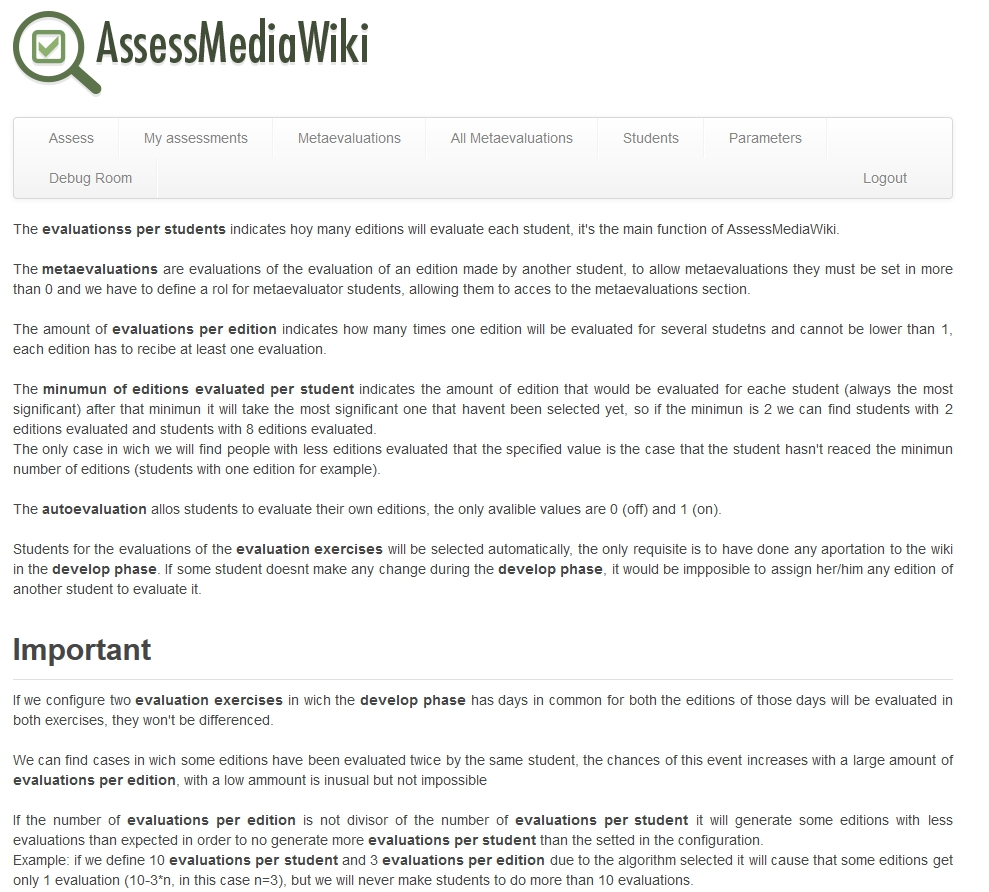
\includegraphics[width=0.9\textwidth]{sc_extra_help.jpg}
	\caption{Pantalla de ayuda extra.}
\end{figure}







\chapter{Conclusiones}
% ------------------------------------------------------------------------------
% Este fichero es parte de la plantilla LaTeX para la realización de Proyectos
% Final de Grado, protegido bajo los términos de la licencia GFDL.
% Para más información, la licencia completa viene incluida en el
% fichero fdl-1.3.tex

% Copyright (C) 2012 SPI-FM. Universidad de Cádiz
% ------------------------------------------------------------------------------

\section{Objetivos alcanzados}
Este apartado debe resumir los objetivos generales y específicos alcanzados, relacionándolos con todo lo descrito en el capítulo de introducción.\\

Se ha podido ampliar las funcionalidades del sistema AssessMediaWiki, añadiendo mas herramientas para los docentes y mas funciones para los alumnos, con la posibilidad de darles responsabilidades personalizadas y haciendo que la experiencia docente sea mas interactiva entre ellos y con el profesor.

\section{Lecciones aprendidas}
A continuación, se detallan las buenas prácticas adquiridas, tanto tecnológicas como procedimentales, así como cualquier otro aspecto de interés.\\

Resumir cuantitativamente el tiempo y esfuerzo dedicados al proyecto a lo largo de su desarrollo que escribir un sencillo 'he trabajado mucho en este proyecto'.
Tras unos nueve meses (a parte de experiencias previas) dedicándole a este proyecto una media de dos horas diarias (o al menos intentándolo) me he dado cuenta de que realmente lanzar una actualización o una nueva versión de algo lleva mucho tiempo y esfuerzo.\\

También he aprendido mucho sobre los framework, buscar recursos por internet y la ayuda de la comunidad en webs como StackOverflow

\section{Trabajo futuro}
En esta sección, se presentan las diversas áreas u oportunidades de mejora detectadas durante el desarrollo del proyecto y que podrán ser abarcadas en futuras versiones del software.\\

Como trabajo futuro quedan pendiente:
\begin{itemize}
	\item Detección de mas wiki-comportamientos, como las ediciones de correcciones ortográficas y desplazamientos de texto.
	\item Realizar preasignaciones se realicen de forma automática (intentando mantener la independencia con el sistema operativo).
	\item Poder trabajar con AssessMediaWiki vía API.
	\item Integración como una extensión de MediaWiki.
	\item Botón de conflicto de interés / rechazar evaluación.
	
	
\end{itemize}

\chapter*{\bibname}
\addcontentsline{toc}{chapter}{\bibname}
%\renewcommand{\bibname}{}

%\input{./bibliografia}

\begingroup
  \def\chapter*#1{}
\renewcommand{\bibname}{}
% Bibliografía con BibTeX
\bibliographystyle{apalike}
\bibliography{bibliografia}

\backmatter

% ------------------------------------------------------------------------------
% Este fichero es parte de la plantilla LaTeX para la realización de Proyectos
% Final de Grado, protegido bajo los términos de la licencia GFDL.
% Para más información, la licencia completa viene incluida en el
% fichero fdl-1.3.tex

% Copyright (C) 2012 SPI-FM. Universidad de Cádiz
% ------------------------------------------------------------------------------


\chapter*{\rlap{Información sobre Licencia}}
\phantomsection  % so hyperref creates bookmarks
\addcontentsline{toc}{chapter}{Información sobre Licencia}
%\label{label_fdl}

 \begin{center}

       Información sobre Licencia


\end{center}

AssessMediaWiki se desarrolla bajo los términos de la licencia GPL.
\newline

Este fichero es parte de la plantilla LaTeX para la realización de Proyectos Final de Grado, protegido bajo los términos de la licencia GFDL (GNU Free Documentation License), se incluyen a continuación los términos de la licencia en ingles. Para más información, la licencia completa viene incluida en el fichero fdl-1.3.tex
\newline

Permission is granted to copy, distribute and/or modify this document under the terms of the GNU Free Documentation License, Version 1.3 or any later version published by the Free Software Foundation; with no Invariant Sections, no Front-Cover Texts, and no Back-Cover Texts. A copy of the license is included in the section entitled "GNU Free Documentation License".
%GNU % ------------------------------------------------------------------------------
% Este fichero es parte de la plantilla LaTeX para la realización de Proyectos
% Final de Grado, protegido bajo los términos de la licencia GFDL.
% Para más información, la licencia completa viene incluida en el
% fichero fdl-1.3.tex

% Copyright (C) 2012 SPI-FM. Universidad de Cádiz
% ------------------------------------------------------------------------------


\chapter*{\rlap{GNU Free Documentation License}}
\phantomsection  % so hyperref creates bookmarks
\addcontentsline{toc}{chapter}{GNU Free Documentation License}
%\label{label_fdl}

 \begin{center}

       Version 1.3, 3 November 2008


 Copyright \copyright{} 2000, 2001, 2002, 2007, 2008  Free Software Foundation, Inc.
 
 \bigskip
 
     <http://fsf.org/>
  
 \bigskip
 
 Everyone is permitted to copy and distribute verbatim copies
 of this license document, but changing it is not allowed.
\end{center}


\begin{center}
{\bf\large Preamble}
\end{center}

The purpose of this License is to make a manual, textbook, or other
functional and useful document ``free'' in the sense of freedom: to
assure everyone the effective freedom to copy and redistribute it,
with or without modifying it, either commercially or noncommercially.
Secondarily, this License preserves for the author and publisher a way
to get credit for their work, while not being considered responsible
for modifications made by others.

This License is a kind of ``copyleft'', which means that derivative
works of the document must themselves be free in the same sense.  It
complements the GNU General Public License, which is a copyleft
license designed for free software.

We have designed this License in order to use it for manuals for free
software, because free software needs free documentation: a free
program should come with manuals providing the same freedoms that the
software does.  But this License is not limited to software manuals;
it can be used for any textual work, regardless of subject matter or
whether it is published as a printed book.  We recommend this License
principally for works whose purpose is instruction or reference.


\begin{center}
{\Large\bf 1. APPLICABILITY AND DEFINITIONS\par}
\phantomsection
\addcontentsline{toc}{section}{1. APPLICABILITY AND DEFINITIONS}
\end{center}

This License applies to any manual or other work, in any medium, that
contains a notice placed by the copyright holder saying it can be
distributed under the terms of this License.  Such a notice grants a
world-wide, royalty-free license, unlimited in duration, to use that
work under the conditions stated herein.  The ``\textbf{Document}'', below,
refers to any such manual or work.  Any member of the public is a
licensee, and is addressed as ``\textbf{you}''.  You accept the license if you
copy, modify or distribute the work in a way requiring permission
under copyright law.

A ``\textbf{Modified Version}'' of the Document means any work containing the
Document or a portion of it, either copied verbatim, or with
modifications and/or translated into another language.

A ``\textbf{Secondary Section}'' is a named appendix or a front-matter section of
the Document that deals exclusively with the relationship of the
publishers or authors of the Document to the Document's overall subject
(or to related matters) and contains nothing that could fall directly
within that overall subject.  (Thus, if the Document is in part a
textbook of mathematics, a Secondary Section may not explain any
mathematics.)  The relationship could be a matter of historical
connection with the subject or with related matters, or of legal,
commercial, philosophical, ethical or political position regarding
them.

The ``\textbf{Invariant Sections}'' are certain Secondary Sections whose titles
are designated, as being those of Invariant Sections, in the notice
that says that the Document is released under this License.  If a
section does not fit the above definition of Secondary then it is not
allowed to be designated as Invariant.  The Document may contain zero
Invariant Sections.  If the Document does not identify any Invariant
Sections then there are none.

The ``\textbf{Cover Texts}'' are certain short passages of text that are listed,
as Front-Cover Texts or Back-Cover Texts, in the notice that says that
the Document is released under this License.  A Front-Cover Text may
be at most 5 words, and a Back-Cover Text may be at most 25 words.

A ``\textbf{Transparent}'' copy of the Document means a machine-readable copy,
represented in a format whose specification is available to the
general public, that is suitable for revising the document
straightforwardly with generic text editors or (for images composed of
pixels) generic paint programs or (for drawings) some widely available
drawing editor, and that is suitable for input to text formatters or
for automatic translation to a variety of formats suitable for input
to text formatters.  A copy made in an otherwise Transparent file
format whose markup, or absence of markup, has been arranged to thwart
or discourage subsequent modification by readers is not Transparent.
An image format is not Transparent if used for any substantial amount
of text.  A copy that is not ``Transparent'' is called ``\textbf{Opaque}''.

Examples of suitable formats for Transparent copies include plain
ASCII without markup, Texinfo input format, LaTeX input format, SGML
or XML using a publicly available DTD, and standard-conforming simple
HTML, PostScript or PDF designed for human modification.  Examples of
transparent image formats include PNG, XCF and JPG.  Opaque formats
include proprietary formats that can be read and edited only by
proprietary word processors, SGML or XML for which the DTD and/or
processing tools are not generally available, and the
machine-generated HTML, PostScript or PDF produced by some word
processors for output purposes only.

The ``\textbf{Title Page}'' means, for a printed book, the title page itself,
plus such following pages as are needed to hold, legibly, the material
this License requires to appear in the title page.  For works in
formats which do not have any title page as such, ``Title Page'' means
the text near the most prominent appearance of the work's title,
preceding the beginning of the body of the text.

The ``\textbf{publisher}'' means any person or entity that distributes
copies of the Document to the public.

A section ``\textbf{Entitled XYZ}'' means a named subunit of the Document whose
title either is precisely XYZ or contains XYZ in parentheses following
text that translates XYZ in another language.  (Here XYZ stands for a
specific section name mentioned below, such as ``\textbf{Acknowledgements}'',
``\textbf{Dedications}'', ``\textbf{Endorsements}'', or ``\textbf{History}''.)  
To ``\textbf{Preserve the Title}''
of such a section when you modify the Document means that it remains a
section ``Entitled XYZ'' according to this definition.

The Document may include Warranty Disclaimers next to the notice which
states that this License applies to the Document.  These Warranty
Disclaimers are considered to be included by reference in this
License, but only as regards disclaiming warranties: any other
implication that these Warranty Disclaimers may have is void and has
no effect on the meaning of this License.


\begin{center}
{\Large\bf 2. VERBATIM COPYING\par}
\phantomsection
\addcontentsline{toc}{section}{2. VERBATIM COPYING}
\end{center}

You may copy and distribute the Document in any medium, either
commercially or noncommercially, provided that this License, the
copyright notices, and the license notice saying this License applies
to the Document are reproduced in all copies, and that you add no other
conditions whatsoever to those of this License.  You may not use
technical measures to obstruct or control the reading or further
copying of the copies you make or distribute.  However, you may accept
compensation in exchange for copies.  If you distribute a large enough
number of copies you must also follow the conditions in section~3.

You may also lend copies, under the same conditions stated above, and
you may publicly display copies.


\begin{center}
{\Large\bf 3. COPYING IN QUANTITY\par}
\phantomsection
\addcontentsline{toc}{section}{3. COPYING IN QUANTITY}
\end{center}


If you publish printed copies (or copies in media that commonly have
printed covers) of the Document, numbering more than 100, and the
Document's license notice requires Cover Texts, you must enclose the
copies in covers that carry, clearly and legibly, all these Cover
Texts: Front-Cover Texts on the front cover, and Back-Cover Texts on
the back cover.  Both covers must also clearly and legibly identify
you as the publisher of these copies.  The front cover must present
the full title with all words of the title equally prominent and
visible.  You may add other material on the covers in addition.
Copying with changes limited to the covers, as long as they preserve
the title of the Document and satisfy these conditions, can be treated
as verbatim copying in other respects.

If the required texts for either cover are too voluminous to fit
legibly, you should put the first ones listed (as many as fit
reasonably) on the actual cover, and continue the rest onto adjacent
pages.

If you publish or distribute Opaque copies of the Document numbering
more than 100, you must either include a machine-readable Transparent
copy along with each Opaque copy, or state in or with each Opaque copy
a computer-network location from which the general network-using
public has access to download using public-standard network protocols
a complete Transparent copy of the Document, free of added material.
If you use the latter option, you must take reasonably prudent steps,
when you begin distribution of Opaque copies in quantity, to ensure
that this Transparent copy will remain thus accessible at the stated
location until at least one year after the last time you distribute an
Opaque copy (directly or through your agents or retailers) of that
edition to the public.

It is requested, but not required, that you contact the authors of the
Document well before redistributing any large number of copies, to give
them a chance to provide you with an updated version of the Document.


\begin{center}
{\Large\bf 4. MODIFICATIONS\par}
\phantomsection
\addcontentsline{toc}{section}{4. MODIFICATIONS}
\end{center}

You may copy and distribute a Modified Version of the Document under
the conditions of sections 2 and 3 above, provided that you release
the Modified Version under precisely this License, with the Modified
Version filling the role of the Document, thus licensing distribution
and modification of the Modified Version to whoever possesses a copy
of it.  In addition, you must do these things in the Modified Version:

\begin{itemize}
\item[A.] 
   Use in the Title Page (and on the covers, if any) a title distinct
   from that of the Document, and from those of previous versions
   (which should, if there were any, be listed in the History section
   of the Document).  You may use the same title as a previous version
   if the original publisher of that version gives permission.
   
\item[B.]
   List on the Title Page, as authors, one or more persons or entities
   responsible for authorship of the modifications in the Modified
   Version, together with at least five of the principal authors of the
   Document (all of its principal authors, if it has fewer than five),
   unless they release you from this requirement.
   
\item[C.]
   State on the Title page the name of the publisher of the
   Modified Version, as the publisher.
   
\item[D.]
   Preserve all the copyright notices of the Document.
   
\item[E.]
   Add an appropriate copyright notice for your modifications
   adjacent to the other copyright notices.
   
\item[F.]
   Include, immediately after the copyright notices, a license notice
   giving the public permission to use the Modified Version under the
   terms of this License, in the form shown in the Addendum below.
   
\item[G.]
   Preserve in that license notice the full lists of Invariant Sections
   and required Cover Texts given in the Document's license notice.
   
\item[H.]
   Include an unaltered copy of this License.
   
\item[I.]
   Preserve the section Entitled ``History'', Preserve its Title, and add
   to it an item stating at least the title, year, new authors, and
   publisher of the Modified Version as given on the Title Page.  If
   there is no section Entitled ``History'' in the Document, create one
   stating the title, year, authors, and publisher of the Document as
   given on its Title Page, then add an item describing the Modified
   Version as stated in the previous sentence.
   
\item[J.]
   Preserve the network location, if any, given in the Document for
   public access to a Transparent copy of the Document, and likewise
   the network locations given in the Document for previous versions
   it was based on.  These may be placed in the ``History'' section.
   You may omit a network location for a work that was published at
   least four years before the Document itself, or if the original
   publisher of the version it refers to gives permission.
   
\item[K.]
   For any section Entitled ``Acknowledgements'' or ``Dedications'',
   Preserve the Title of the section, and preserve in the section all
   the substance and tone of each of the contributor acknowledgements
   and/or dedications given therein.
   
\item[L.]
   Preserve all the Invariant Sections of the Document,
   unaltered in their text and in their titles.  Section numbers
   or the equivalent are not considered part of the section titles.
   
\item[M.]
   Delete any section Entitled ``Endorsements''.  Such a section
   may not be included in the Modified Version.
   
\item[N.]
   Do not retitle any existing section to be Entitled ``Endorsements''
   or to conflict in title with any Invariant Section.
   
\item[O.]
   Preserve any Warranty Disclaimers.
\end{itemize}

If the Modified Version includes new front-matter sections or
appendices that qualify as Secondary Sections and contain no material
copied from the Document, you may at your option designate some or all
of these sections as invariant.  To do this, add their titles to the
list of Invariant Sections in the Modified Version's license notice.
These titles must be distinct from any other section titles.

You may add a section Entitled ``Endorsements'', provided it contains
nothing but endorsements of your Modified Version by various
parties---for example, statements of peer review or that the text has
been approved by an organization as the authoritative definition of a
standard.

You may add a passage of up to five words as a Front-Cover Text, and a
passage of up to 25 words as a Back-Cover Text, to the end of the list
of Cover Texts in the Modified Version.  Only one passage of
Front-Cover Text and one of Back-Cover Text may be added by (or
through arrangements made by) any one entity.  If the Document already
includes a cover text for the same cover, previously added by you or
by arrangement made by the same entity you are acting on behalf of,
you may not add another; but you may replace the old one, on explicit
permission from the previous publisher that added the old one.

The author(s) and publisher(s) of the Document do not by this License
give permission to use their names for publicity for or to assert or
imply endorsement of any Modified Version.


\begin{center}
{\Large\bf 5. COMBINING DOCUMENTS\par}
\phantomsection
\addcontentsline{toc}{section}{5. COMBINING DOCUMENTS}
\end{center}


You may combine the Document with other documents released under this
License, under the terms defined in section~4 above for modified
versions, provided that you include in the combination all of the
Invariant Sections of all of the original documents, unmodified, and
list them all as Invariant Sections of your combined work in its
license notice, and that you preserve all their Warranty Disclaimers.

The combined work need only contain one copy of this License, and
multiple identical Invariant Sections may be replaced with a single
copy.  If there are multiple Invariant Sections with the same name but
different contents, make the title of each such section unique by
adding at the end of it, in parentheses, the name of the original
author or publisher of that section if known, or else a unique number.
Make the same adjustment to the section titles in the list of
Invariant Sections in the license notice of the combined work.

In the combination, you must combine any sections Entitled ``History''
in the various original documents, forming one section Entitled
``History''; likewise combine any sections Entitled ``Acknowledgements'',
and any sections Entitled ``Dedications''.  You must delete all sections
Entitled ``Endorsements''.

\begin{center}
{\Large\bf 6. COLLECTIONS OF DOCUMENTS\par}
\phantomsection
\addcontentsline{toc}{section}{6. COLLECTIONS OF DOCUMENTS}
\end{center}

You may make a collection consisting of the Document and other documents
released under this License, and replace the individual copies of this
License in the various documents with a single copy that is included in
the collection, provided that you follow the rules of this License for
verbatim copying of each of the documents in all other respects.

You may extract a single document from such a collection, and distribute
it individually under this License, provided you insert a copy of this
License into the extracted document, and follow this License in all
other respects regarding verbatim copying of that document.


\begin{center}
{\Large\bf 7. AGGREGATION WITH INDEPENDENT WORKS\par}
\phantomsection
\addcontentsline{toc}{section}{7. AGGREGATION WITH INDEPENDENT WORKS}
\end{center}


A compilation of the Document or its derivatives with other separate
and independent documents or works, in or on a volume of a storage or
distribution medium, is called an ``aggregate'' if the copyright
resulting from the compilation is not used to limit the legal rights
of the compilation's users beyond what the individual works permit.
When the Document is included in an aggregate, this License does not
apply to the other works in the aggregate which are not themselves
derivative works of the Document.

If the Cover Text requirement of section~3 is applicable to these
copies of the Document, then if the Document is less than one half of
the entire aggregate, the Document's Cover Texts may be placed on
covers that bracket the Document within the aggregate, or the
electronic equivalent of covers if the Document is in electronic form.
Otherwise they must appear on printed covers that bracket the whole
aggregate.


\begin{center}
{\Large\bf 8. TRANSLATION\par}
\phantomsection
\addcontentsline{toc}{section}{8. TRANSLATION}
\end{center}


Translation is considered a kind of modification, so you may
distribute translations of the Document under the terms of section~4.
Replacing Invariant Sections with translations requires special
permission from their copyright holders, but you may include
translations of some or all Invariant Sections in addition to the
original versions of these Invariant Sections.  You may include a
translation of this License, and all the license notices in the
Document, and any Warranty Disclaimers, provided that you also include
the original English version of this License and the original versions
of those notices and disclaimers.  In case of a disagreement between
the translation and the original version of this License or a notice
or disclaimer, the original version will prevail.

If a section in the Document is Entitled ``Acknowledgements'',
``Dedications'', or ``History'', the requirement (section~4) to Preserve
its Title (section~1) will typically require changing the actual
title.


\begin{center}
{\Large\bf 9. TERMINATION\par}
\phantomsection
\addcontentsline{toc}{section}{9. TERMINATION}
\end{center}


You may not copy, modify, sublicense, or distribute the Document
except as expressly provided under this License.  Any attempt
otherwise to copy, modify, sublicense, or distribute it is void, and
will automatically terminate your rights under this License.

However, if you cease all violation of this License, then your license
from a particular copyright holder is reinstated (a) provisionally,
unless and until the copyright holder explicitly and finally
terminates your license, and (b) permanently, if the copyright holder
fails to notify you of the violation by some reasonable means prior to
60 days after the cessation.

Moreover, your license from a particular copyright holder is
reinstated permanently if the copyright holder notifies you of the
violation by some reasonable means, this is the first time you have
received notice of violation of this License (for any work) from that
copyright holder, and you cure the violation prior to 30 days after
your receipt of the notice.

Termination of your rights under this section does not terminate the
licenses of parties who have received copies or rights from you under
this License.  If your rights have been terminated and not permanently
reinstated, receipt of a copy of some or all of the same material does
not give you any rights to use it.


\begin{center}
{\Large\bf 10. FUTURE REVISIONS OF THIS LICENSE\par}
\phantomsection
\addcontentsline{toc}{section}{10. FUTURE REVISIONS OF THIS LICENSE}
\end{center}


The Free Software Foundation may publish new, revised versions
of the GNU Free Documentation License from time to time.  Such new
versions will be similar in spirit to the present version, but may
differ in detail to address new problems or concerns.  See
http://www.gnu.org/copyleft/.

Each version of the License is given a distinguishing version number.
If the Document specifies that a particular numbered version of this
License ``or any later version'' applies to it, you have the option of
following the terms and conditions either of that specified version or
of any later version that has been published (not as a draft) by the
Free Software Foundation.  If the Document does not specify a version
number of this License, you may choose any version ever published (not
as a draft) by the Free Software Foundation.  If the Document
specifies that a proxy can decide which future versions of this
License can be used, that proxy's public statement of acceptance of a
version permanently authorizes you to choose that version for the
Document.


\begin{center}
{\Large\bf 11. RELICENSING\par}
\phantomsection
\addcontentsline{toc}{section}{11. RELICENSING}
\end{center}


``Massive Multiauthor Collaboration Site'' (or ``MMC Site'') means any
World Wide Web server that publishes copyrightable works and also
provides prominent facilities for anybody to edit those works.  A
public wiki that anybody can edit is an example of such a server.  A
``Massive Multiauthor Collaboration'' (or ``MMC'') contained in the
site means any set of copyrightable works thus published on the MMC
site.

``CC-BY-SA'' means the Creative Commons Attribution-Share Alike 3.0
license published by Creative Commons Corporation, a not-for-profit
corporation with a principal place of business in San Francisco,
California, as well as future copyleft versions of that license
published by that same organization.

``Incorporate'' means to publish or republish a Document, in whole or
in part, as part of another Document.

An MMC is ``eligible for relicensing'' if it is licensed under this
License, and if all works that were first published under this License
somewhere other than this MMC, and subsequently incorporated in whole
or in part into the MMC, (1) had no cover texts or invariant sections,
and (2) were thus incorporated prior to November 1, 2008.

The operator of an MMC Site may republish an MMC contained in the site
under CC-BY-SA on the same site at any time before August 1, 2009,
provided the MMC is eligible for relicensing.


\begin{center}
{\Large\bf ADDENDUM: How to use this License for your documents\par}
\phantomsection
\addcontentsline{toc}{section}{ADDENDUM: How to use this License for your documents}
\end{center}

To use this License in a document you have written, include a copy of
the License in the document and put the following copyright and
license notices just after the title page:

\bigskip
\begin{quote}
    Copyright \copyright{}  YEAR  YOUR NAME.
    Permission is granted to copy, distribute and/or modify this document
    under the terms of the GNU Free Documentation License, Version 1.3
    or any later version published by the Free Software Foundation;
    with no Invariant Sections, no Front-Cover Texts, and no Back-Cover Texts.
    A copy of the license is included in the section entitled ``GNU
    Free Documentation License''.
\end{quote}
\bigskip
    
If you have Invariant Sections, Front-Cover Texts and Back-Cover Texts,
replace the ``with \dots\ Texts.'' line with this:

\bigskip
\begin{quote}
    with the Invariant Sections being LIST THEIR TITLES, with the
    Front-Cover Texts being LIST, and with the Back-Cover Texts being LIST.
\end{quote}
\bigskip
    
If you have Invariant Sections without Cover Texts, or some other
combination of the three, merge those two alternatives to suit the
situation.

If your document contains nontrivial examples of program code, we
recommend releasing these examples in parallel under your choice of
free software license, such as the GNU General Public License,
to permit their use in free software.

%---------------------------------------------------------------------


\end{document}
